%from chapin2013:  An individual bolometer acts as a thermal absorber which are linked directly to transition edge sensors.  When the sensors detect detect thermal variations they will produce changing currents which result in changing magnetic fields.  The magnetic fields are detected by super conduction quantum interference devices (SQUIDs) prior to the output currents being digitized.  Between the initial SQUID amplification and digitization of the current, the data is resampled from 12KHz to 200Hz.  A chain of ``dark SQUIDs'' is used to detect any non-thermal noise that can arise from the amplification of the signal.  //all unnecessary....
\chapter{Observations and Data Preparation}\label{observations}

\section{SCUBA-2} \\
The Submillimetre Common-User Bolometer Array 2 (SCUBA-2) was designed to decrease the observing time of the sub-millimetre sky relative to its predecessor SCUBA.  This woule benefit the community by allowing for rapid data acquisition in the submillimetre regime of the electromagnetic spectrum, at the 450$\mu$m and 850$\mu$m bands in particular.  Prior to SCUBA-2, other bolometer camera's such as LABOCA, BOLOCAM and SHARC-II were limited to less than 100 pixels, while the new SCUBA-2 has been able to incorporate over 10,000 pixels in its design and effectively reduce the required observing time.  Increasing the amount of pixels by a factor of 100 was possible by the advent of new technology such as high precision micromachining, superconducting transition edge sensors, and superconducting quantum interference device amplifiers (SQUIDs) \citet{holland2013}.

The observations of NGC3627 were taken from the Nearby Galaxies Legacy Survey's (NGLS) initial science images using SCUBA-2 from December 29, 2011  to January 21, 2012, and consist of 24 18$\arcmin$ by 18$\arcmin$ scans taken in grade 3 weather or better $(0.08 < \tau <0.12)$ with observations centered at 450$\mu$m and 850$\mu$m emission with a 32$\mu$m and 85$\mu$m bandpass respectively.  16 of the 24 scans were deemed useable, and whether or not an observation was deemed worthwhile was determined by factors such as the behavior of the image background or whether the image was flagged in observing to be unusable.  The observations of NGC3627 were taken using a daisy scanning pattern at 150$\arcsec$/second in order to reduce the white noise of the final data product. 

\section{Image Creation and Properties}

For any imaging process to have been successful, the image needed to have limited white noise (\citet{chapin2013}).  White noise in the sense of our bolometer observations arose from thermal variations in the instrument and atmosphere during data acquisition. The random noise can be minimized through scanning methods and during image processing \citet{chapin2013}.  To create the final SCUBA-2 data products we used the Submillimetre User Reduction Facility (SMURF) procedure MAKEMAP.  This procedure reduced the noise of the observations while maintaining the source's emission by incorporating a combination of principal component analysis and a maximum likelihood analysis \citet{chapin2013}.  Both of these methods have proven useful in reducing bolometer data on their own, but due to the size of raw SCUBA-2 data, either method on its own would have resulted in extreme run times or the process becoming resource intensive.

MAKEMAP broke down the image creation into several steps performed in iteration in order to successfully reduce any background noise (\citet{chapin2013}).  The steps used in MAKEMAP were:  COM and GAI which remove any common noise features detected by the SQUIDs, EXT to apply extinction corrections, FLT applied  a high- and low-pass filters to remove any noise features not removed in the COM and GAI filtering, AST which regrids the data and detects sources to be removed from reduction, the final step is NOI which determines the noise in the gridded map after each step has been performed.  A convergence check is then issued and if the check failed the COM, GAI, EXT, and FLT values are inverted and the process is repeated with the inverted values (\citet{chapin2013}).

In our production of maps, we used the conifguration file dimmconfig\_bright\_compact.lis and altered the AST and FLT sections of the image creation by introducing a mask made from Herschel's 250$\mu$m map.  The purpose of the map was to exclude the target from interfering with the noise minimization as well as prohibit any emission from the galaxy to be significantly altered during image production.  The filter size of the high-pass filter was also modified, and an appropriate value was determined to be 175$\arcsec$.  The maps were returned from MAKEMAP in units of pW with a pixel size of 2$\arcsec$ by 2$\arcsec$ for both the 450$\mu$m and 850$\mu$m.

The finalized 450$\mu$m image was then re-gridded down to a 4$\arcsec$ by 4$\arcsec$ pixel grid, and a flux calibration value of 491000 and 4710 were applied to convert from pW to mJy/beam and mJy/square arcsecond respectively.  The 850$\mu$m maps were re-gridded to an 8$\arcsec$ by 8$\arcsec$ pixel size and used flux calibration values of 537000 and 2340 for mJy/beam and mJy/square arcsecond.  The 4$\arcsec$  and 8$\arcsec$ pixels corresponed to a 10kpc and 20kpc size scale for our target, NGC3627.  To simplify the analysis, the images were also converted to Jy/pixel by multiplying the mJy/square arcsecond by 0.001/pixel area.  Both the 450$\mu$m and 850$\mu$m are shown in figures \ref{fig_450} and \ref{fig_850}.  The calibration values were determined from calibrator sources, and for our observations the source was Uranus.   The overall noise in the finalized image scan be seen in table \ref{tab_obs_scuba2}.

\begin{figure}
  \centering
  \label{fig_450}
  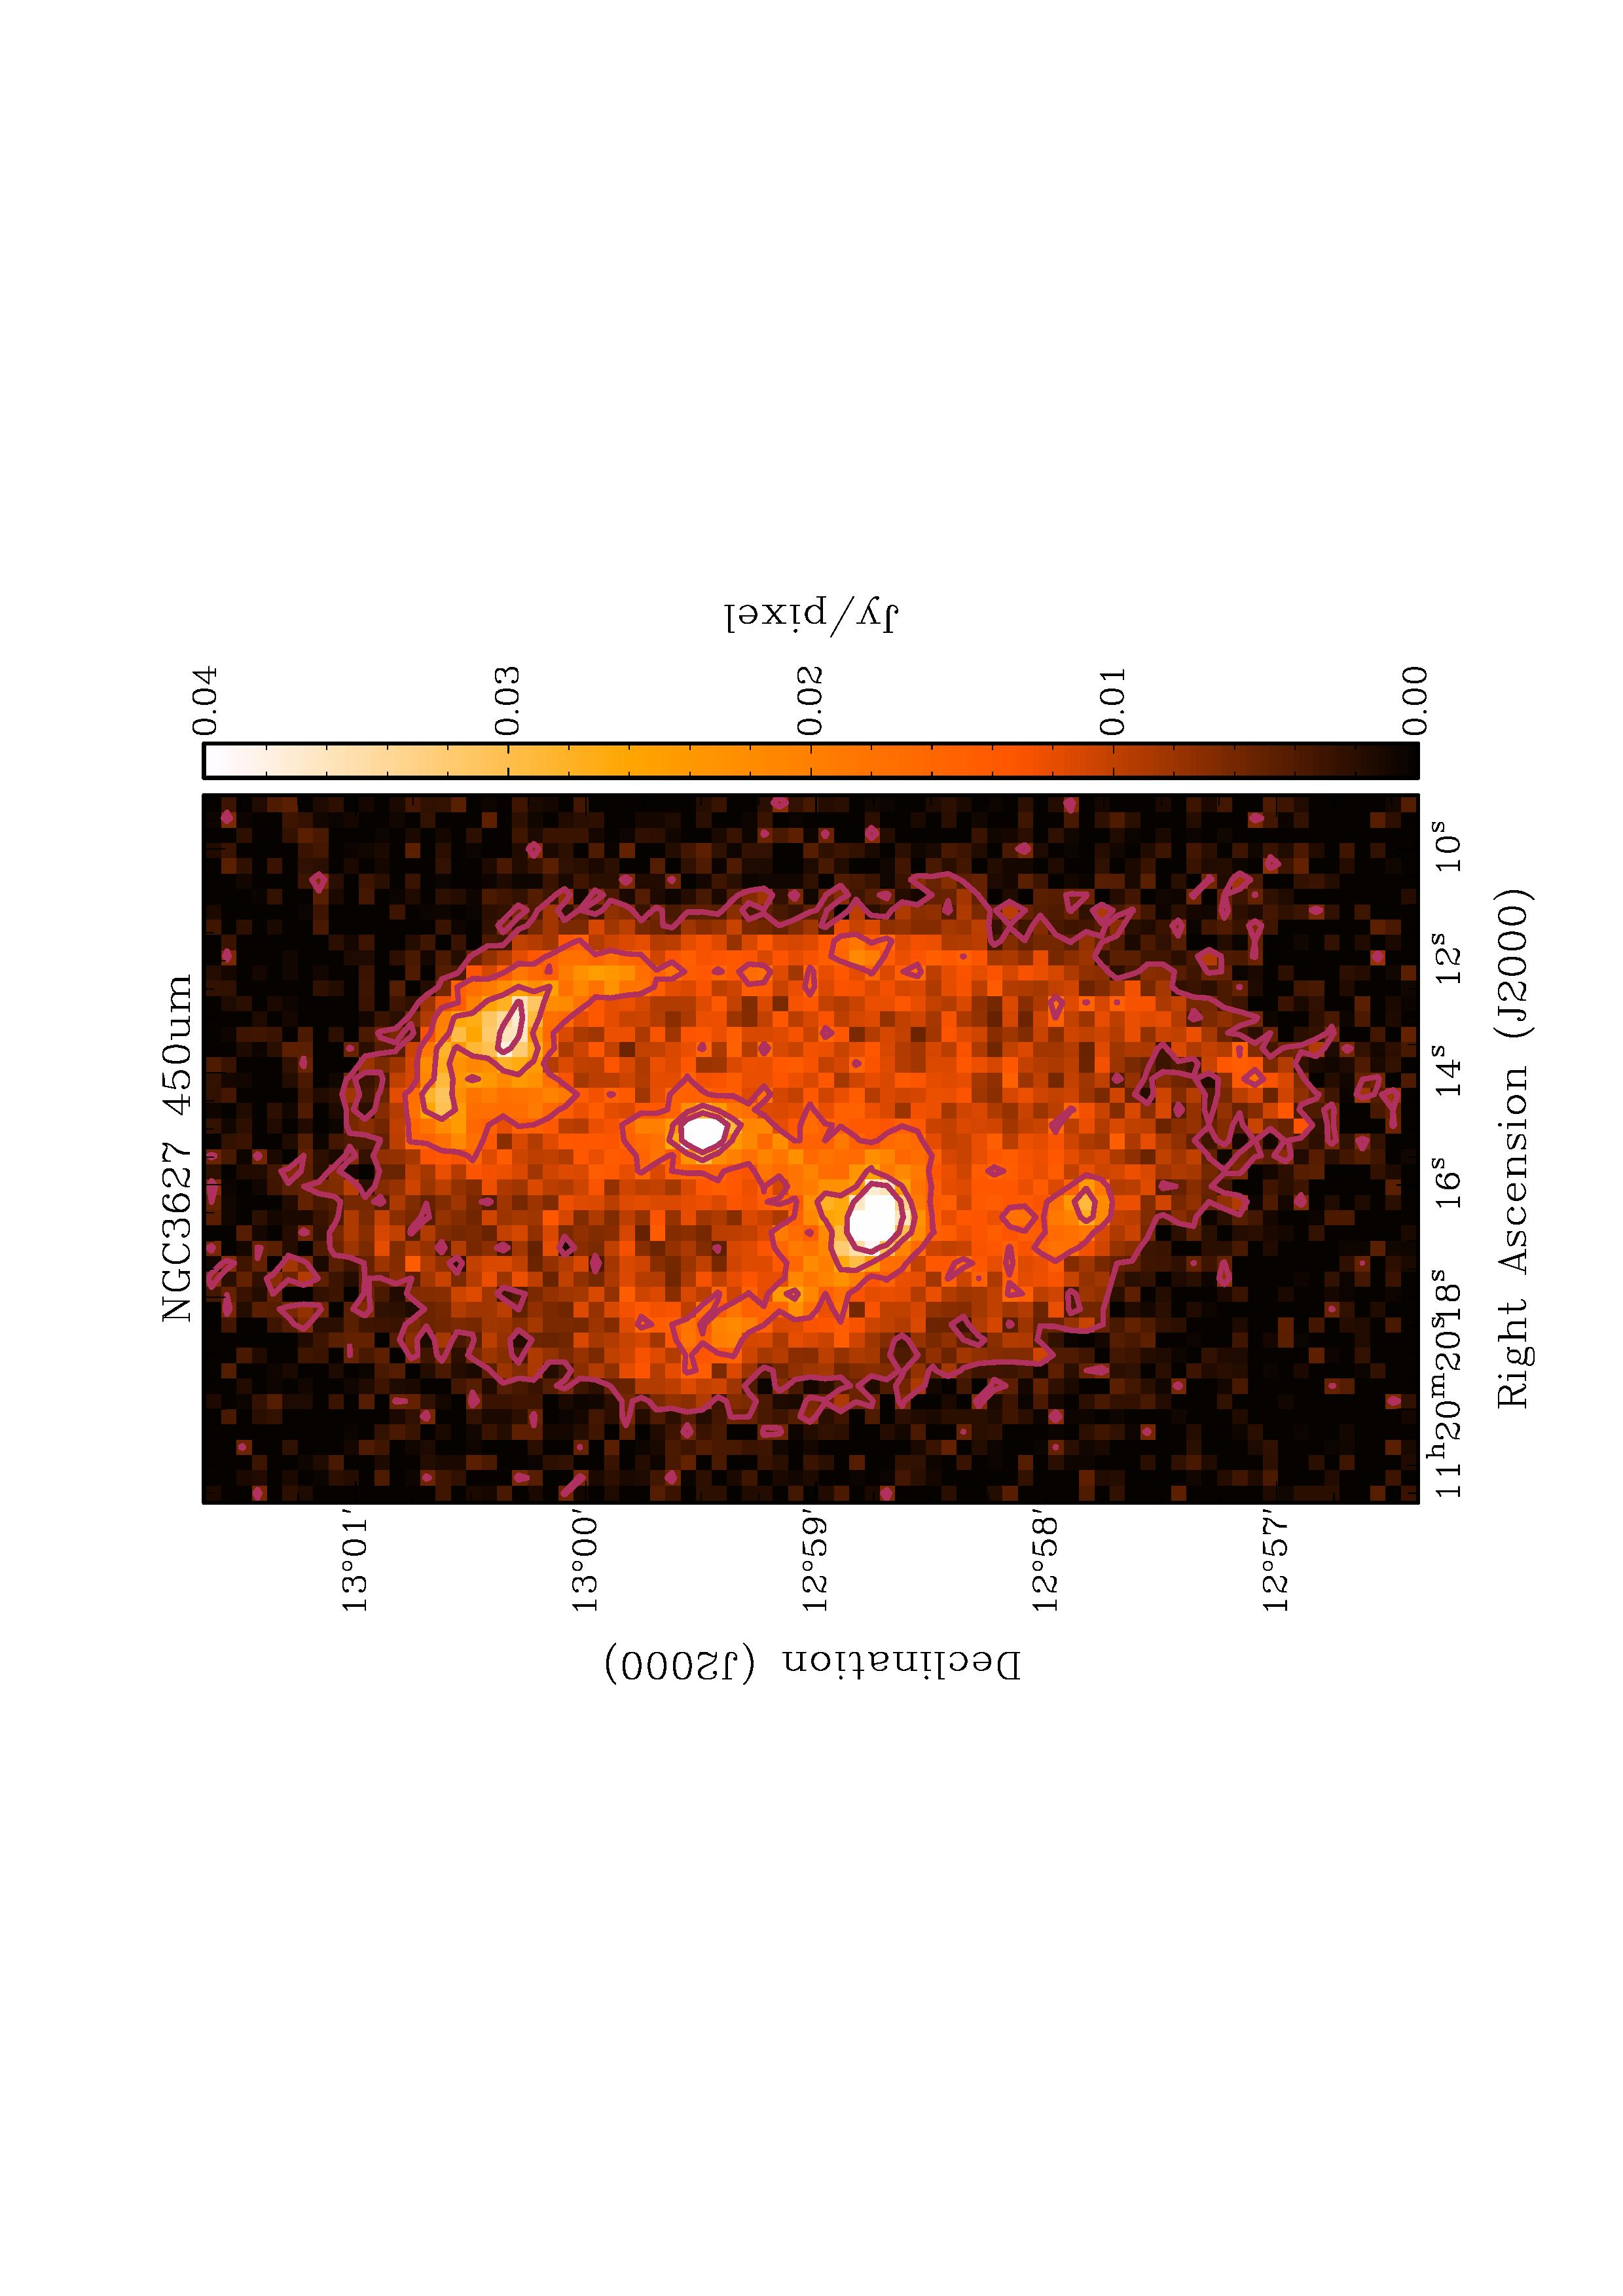
\includegraphics[scale=0.5,angle=270]{obs_imgs/450_um.jpeg}
  \caption[NGC3627 450$\mu$m Observations]{450$\mu$m observation produced at the end of the image production.}
\end{figure}

\begin{figure}
  \centering
  \label{fig_850}
  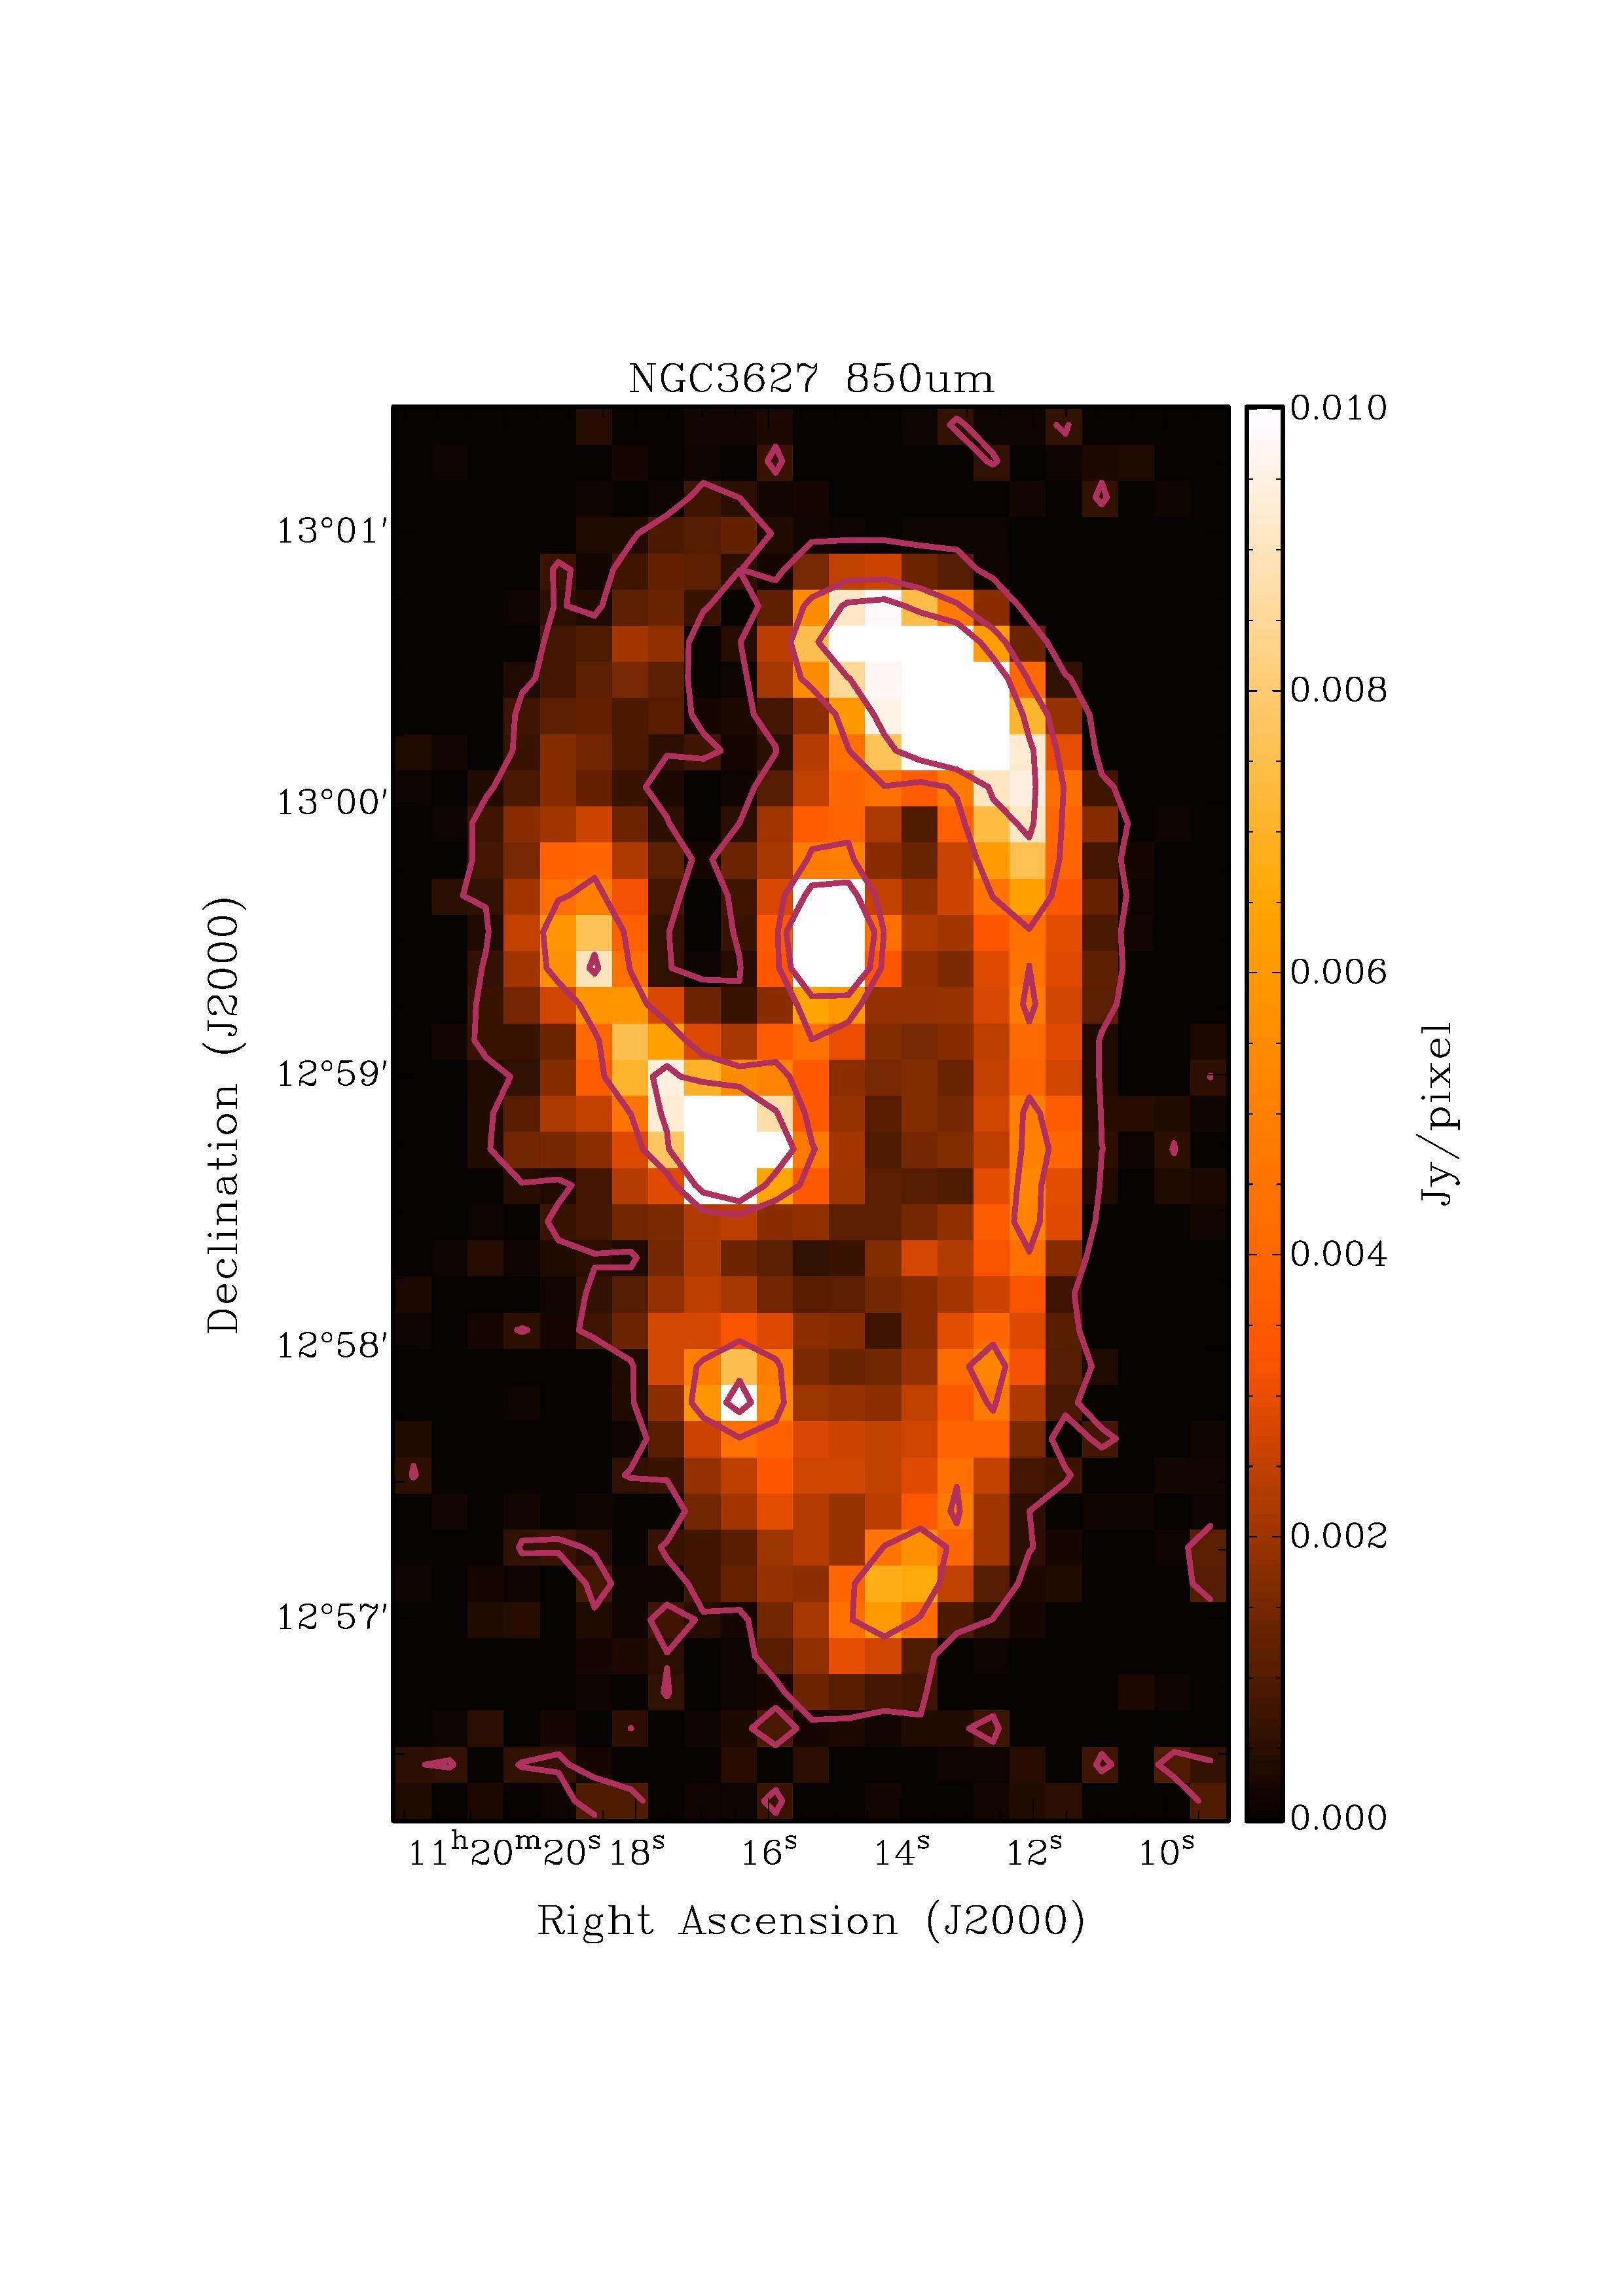
\includegraphics[scale=0.5]{obs_imgs/850_um.jpeg}
  \caption[NGC3627 850$\mu$m Observations]{850$\mu$m observation produced at the end of the image production.}
\end{figure}

\begin{deluxetable}{cccccc}
%  \tabletypesize{\footnotesize}
  \tablecolumns{6}
  \tablewidth{0pt}
  \tablecaption{Properties of NGC3627 SCUBA-2 Observations\label{tab_obs_scuba2}}
  \tablehead{\colhead{Observation} & \multicolumn{4}{c}{Beam Properties} & \colhead{RMS} \\
& $\alpha$ & $\theta_{\alpha}$ & $\beta$ & $\theta_{\beta}$ & \it{[Jy / Pixel]}}
  \startdata
    450$\mu$m & 0.854 & 7.48$\arcsec$ & 0.146 & 23.1$\arcsec$ & 3.42e-3  \\
    850$\mu$m & 0.962 & 12.8$\arcsec$  & 0.038 & 44.5$\arcsec$ &  4.76e-4 \\
   \enddata
\end{deluxetable}

\subsection{Beam Shape of the 450$\mu$m and 850$\mu$m} \\
The Uranus calibration images were also used in determining the shape of the beam for the 450$\mu$m and 850$\mu$m observations.  The beam shape of both the 450$\mu$m and 850$\mu$m deviate from a single gaussian due to the second maximum of the airy diffraction pattern in the response function of the telescope.  This abnormality was best represented by a sum of two gaussians whose amplitude totals to unity \citet{dempsey2013}.  The average beam resolution for the 450$\mu$m and 850$\mu$m are reported in table \ref{tab_obs_scuba2} and match the values within error found in \citet{dempsey2013}.  The calibration images and beams can be seen in figure \ref{fig_calib}.  The contribution of the error beam in the 850$\mu$m emission was negligible and allowed for the beam to be approximated by a single gaussian however the contribution of the error beam in the 450$\mu$m images was large enough to require special treatment.

\begin{figure}
  \label{fig_calib}
  \centering
  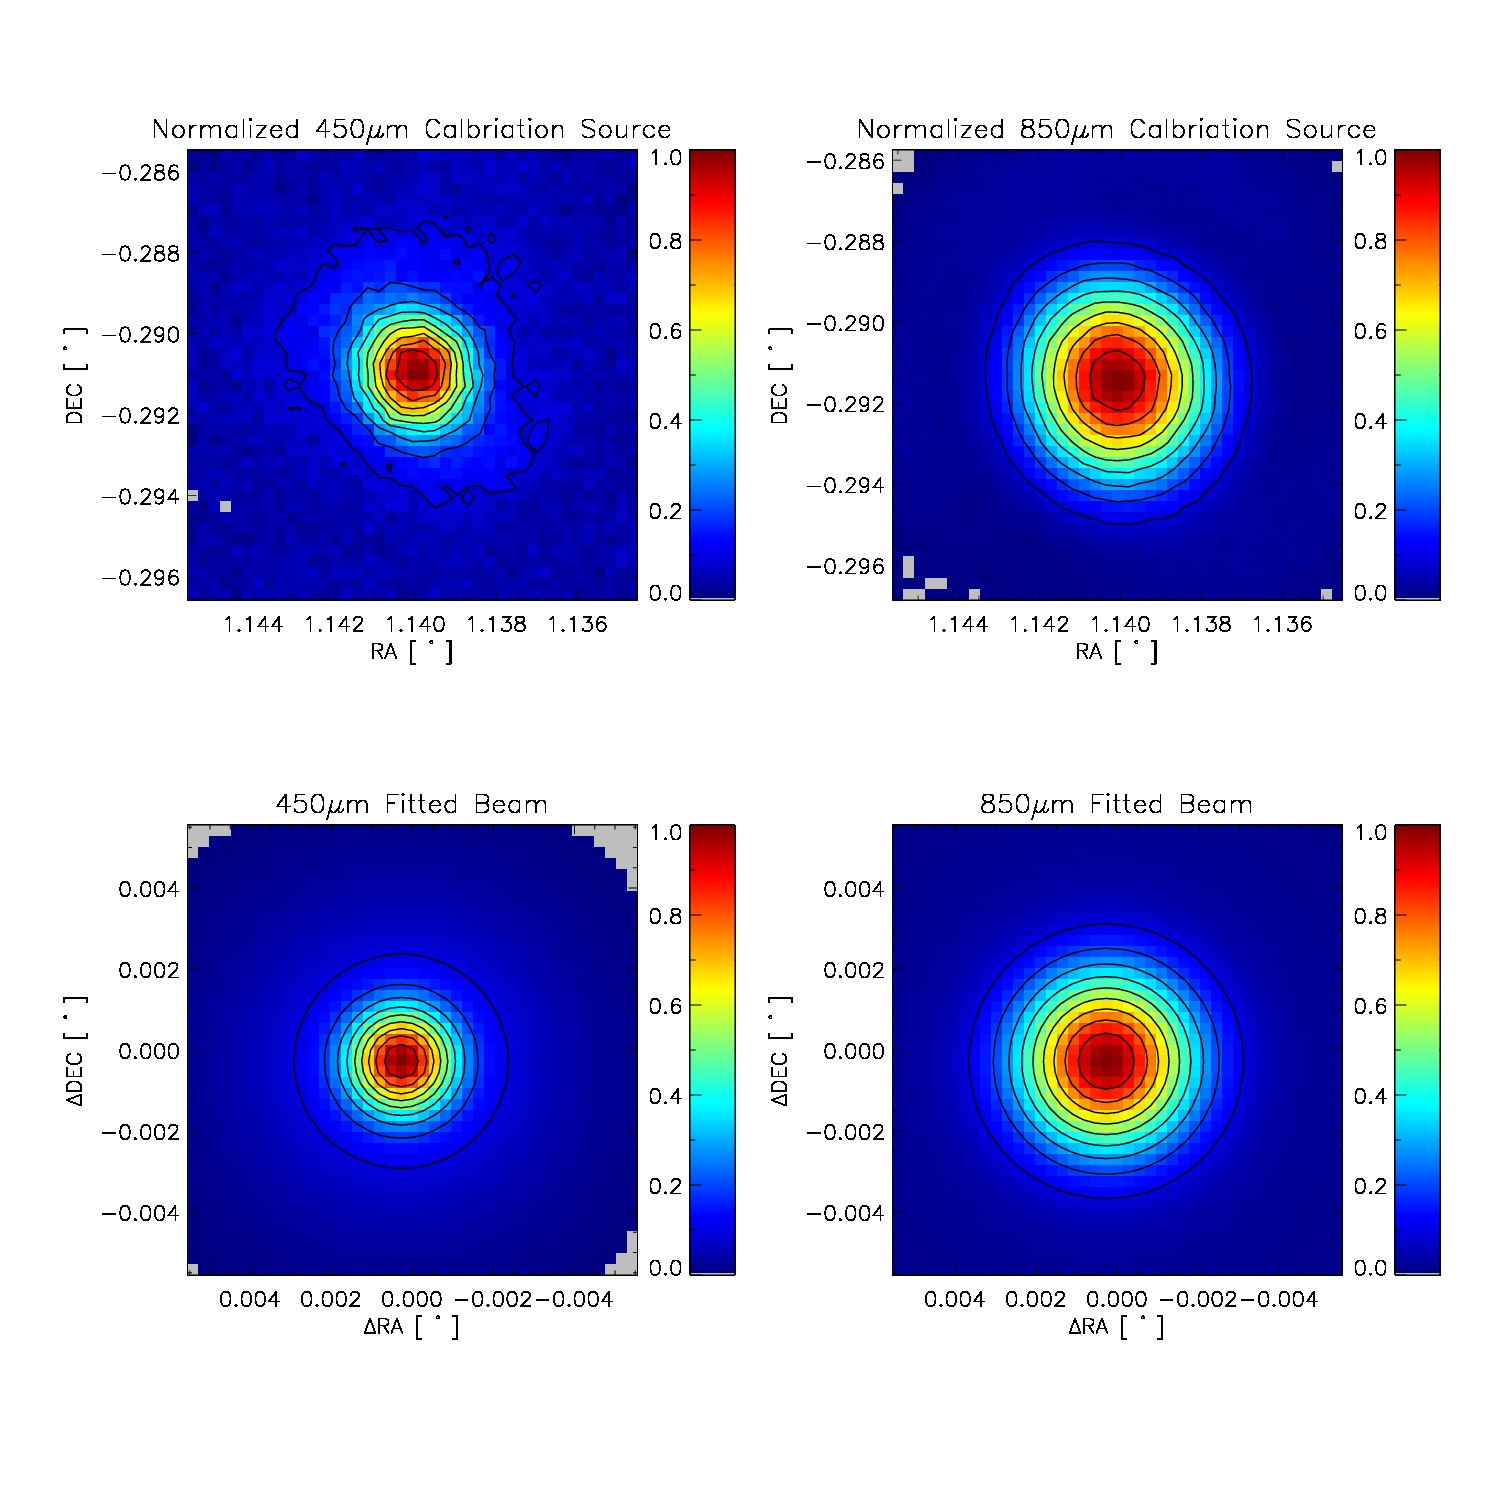
\includegraphics[scale=0.5]{obs_imgs/calib_beams.jpeg}
  \caption[SCUBA-2 Calibration and Beams]{The top row shows the Uranus images taken on January, 5th 2012 for the 450$\mu$m on the left and the 850$\mu$m on the right.  The bottom row shows the fitted beams for the 450$\mu$m on the right and 850$\mu$m on the left using the double gaussian beam shape.}
\end{figure}

In order to accommodate the 450$\mu$m's error component, we used a method employed by another SCUBA-2 survey, the Gould-Belt Survey team.  This method utilized the distributive nature of the Fourier transform to create similar error components in the beam resolutions we were convolving to and from.  This relationship is shown in equation \ref{eq_GBSmethod} where $X_{desire}$ is the beam width of the resolution we are convolving to, $\alpha$ is the amplitude of the main beam of the 450$\mu$m emission, $\beta$ is the amplitude of the 450$\mu$m error beam, $X_{\alpha}$ and $X_{\beta}$ are the main and error beam of the 450$\mu$m observations, and $X_{450\mu m}$ is the composition of $X_{\alpha}$ and $X_{\beta}$ beams.

\begin{equation} \label{eq_GBSmethod}
  \left(X_{desire} \ast X_{\alpha}\right)*\alpha + \left(X_{desire} \ast X_{\beta}\right)*\beta = X_{450\mu m} \ast X_{desire}
\end{equation}

\section{Ancillary Data}

The science goals of this thesis required data outside the capabilities of SCUBA-2.  For instance, accurtely determining the dust mass involved fitting the spectral energy distribution (SED) for NGC3627.  To successfully fit an SED, we needed shorter wavelength data to fully probe the cold component of this galaxy. We used data ranging from 100$\mu$m to 500$\mu$m from the KINGFISH survey (\citet{kennicutt2011}) to gain a large enough wavelength range for fitting the cold component.  Secondly, the bandpass of the 850$\mu$m emisison contains the $CO_{j=3-2}$ transmission line.  In order to get a valid approximation on the dust mass, this contribution had to be removed.  We used emisison data from the NGLS using HARP instrumentation on the JCMT \citet{wilson2012}.  When a dust mass was obtained, we used $CO_{j=1-0}$ from the Nobeyama 45-m telescope (\citet{kuno2007}), $CO_{j=2-1}$ from HERACLES (\citet{leroy2009}), and $HI$ observations from THINGS (\citet{walter2008}) to determine an reasonable molecular hydrogen mass to approximate a dust-to-gas ratio.

Due to the combination of methods used in MAKEMAP, small scale/extended structure is removed from the final SCUBA-2 images.  However, in all of our ancillary data the small scale emission was present in the initial maps.  The removal of the extended features from our support data was carried out by either converting the images from their native units into pW using the 850$\mu$m flux calibration factor or by introducing a scaling factor.  The images were overlaid on the original scans as a fakesource and passed through the reduction process.  The original scan was then subtracted from the scan with the fakesource present and the residual of the process was the ancillary data with its extended structure removed.

\subsection{Key Insights on Nearby Galaxies: a Far-Infrared Survey with Herschel (KINGFISH)}

%sings paper not showing up

The Key Insights on Nearby Galaxies: a Far-Infrared Survey with Herschel (KINGSFISH) was designed to be a follow up to the Spitzer Infrared Nearby Galaxies Survey (SINGS) \citet{kennicutt2003} with observations of the warm and cold component of dust emission using the increased resolution from Herschel \citet{kennicutt2011}.  The main science goals of the KINGFISH survey were to better understand the star formation processes that were shielded by dust, resolved studies of heating and cooling of the interstellar medium (ISM), and to build an inventory of how cold dust emission relates to other dust components in the ISM \citet{kennicutt2011}.  The survey consisted of studying 61 nearby galaxies (d$<$30Mpc) that cover a range of environments each observed at 70$\mu$m, 100$\mu$m, 160$\mu$m, 250$\mu$m, 350$\mu$m, and 500$\mu$m.  

We were interested in fitting the cold component of NGC3627's SED, hence we omitted the 70$\mu$m emission, and used the 100$\mu$m, 160$\mu$m, 250$\mu$m, 350$\mu$m and 500$\mu$m.  Since the Kingfish data was acquired by a space-based telescope, a significant amount of small scale emission was recovered due to the lack of interference from the atmosphere.  The small scale emission was removed by treating the KINGFISH data as a fakesource in the image reduction process.  The first step to successfully incorporating the data as a fakesource was to convert the 250$\mu$m, 350$\mu$m, and 500$\mu$m from MJy/sr to mJy/square arcsecond, and similarly the 100$\mu$m and 160$\mu$m from Jy/pixel to mJy/square arcsecond.   After the unit conversion, the 850$\mu$m flux calibration factor was applied in reverse, and the new image was then scaled down to better mimic the 850$\mu$m emission.  After these steps the image was passed into MAKEMAP and treated as an 850$\mu$m image.  The final data output were gridded to 8$\arcsec$ x 8$\arcsec$ pixels correspoding to a 20kpc scale.  The outputted images can be seen in figures \ref{fig_100} through \ref{fig_500}.  The beam size and rms for each image after it has been passed through make map can be seen in table \ref{tab_obs_kfish}.

\begin{figure}
  \centering
  \label{fig_100}
  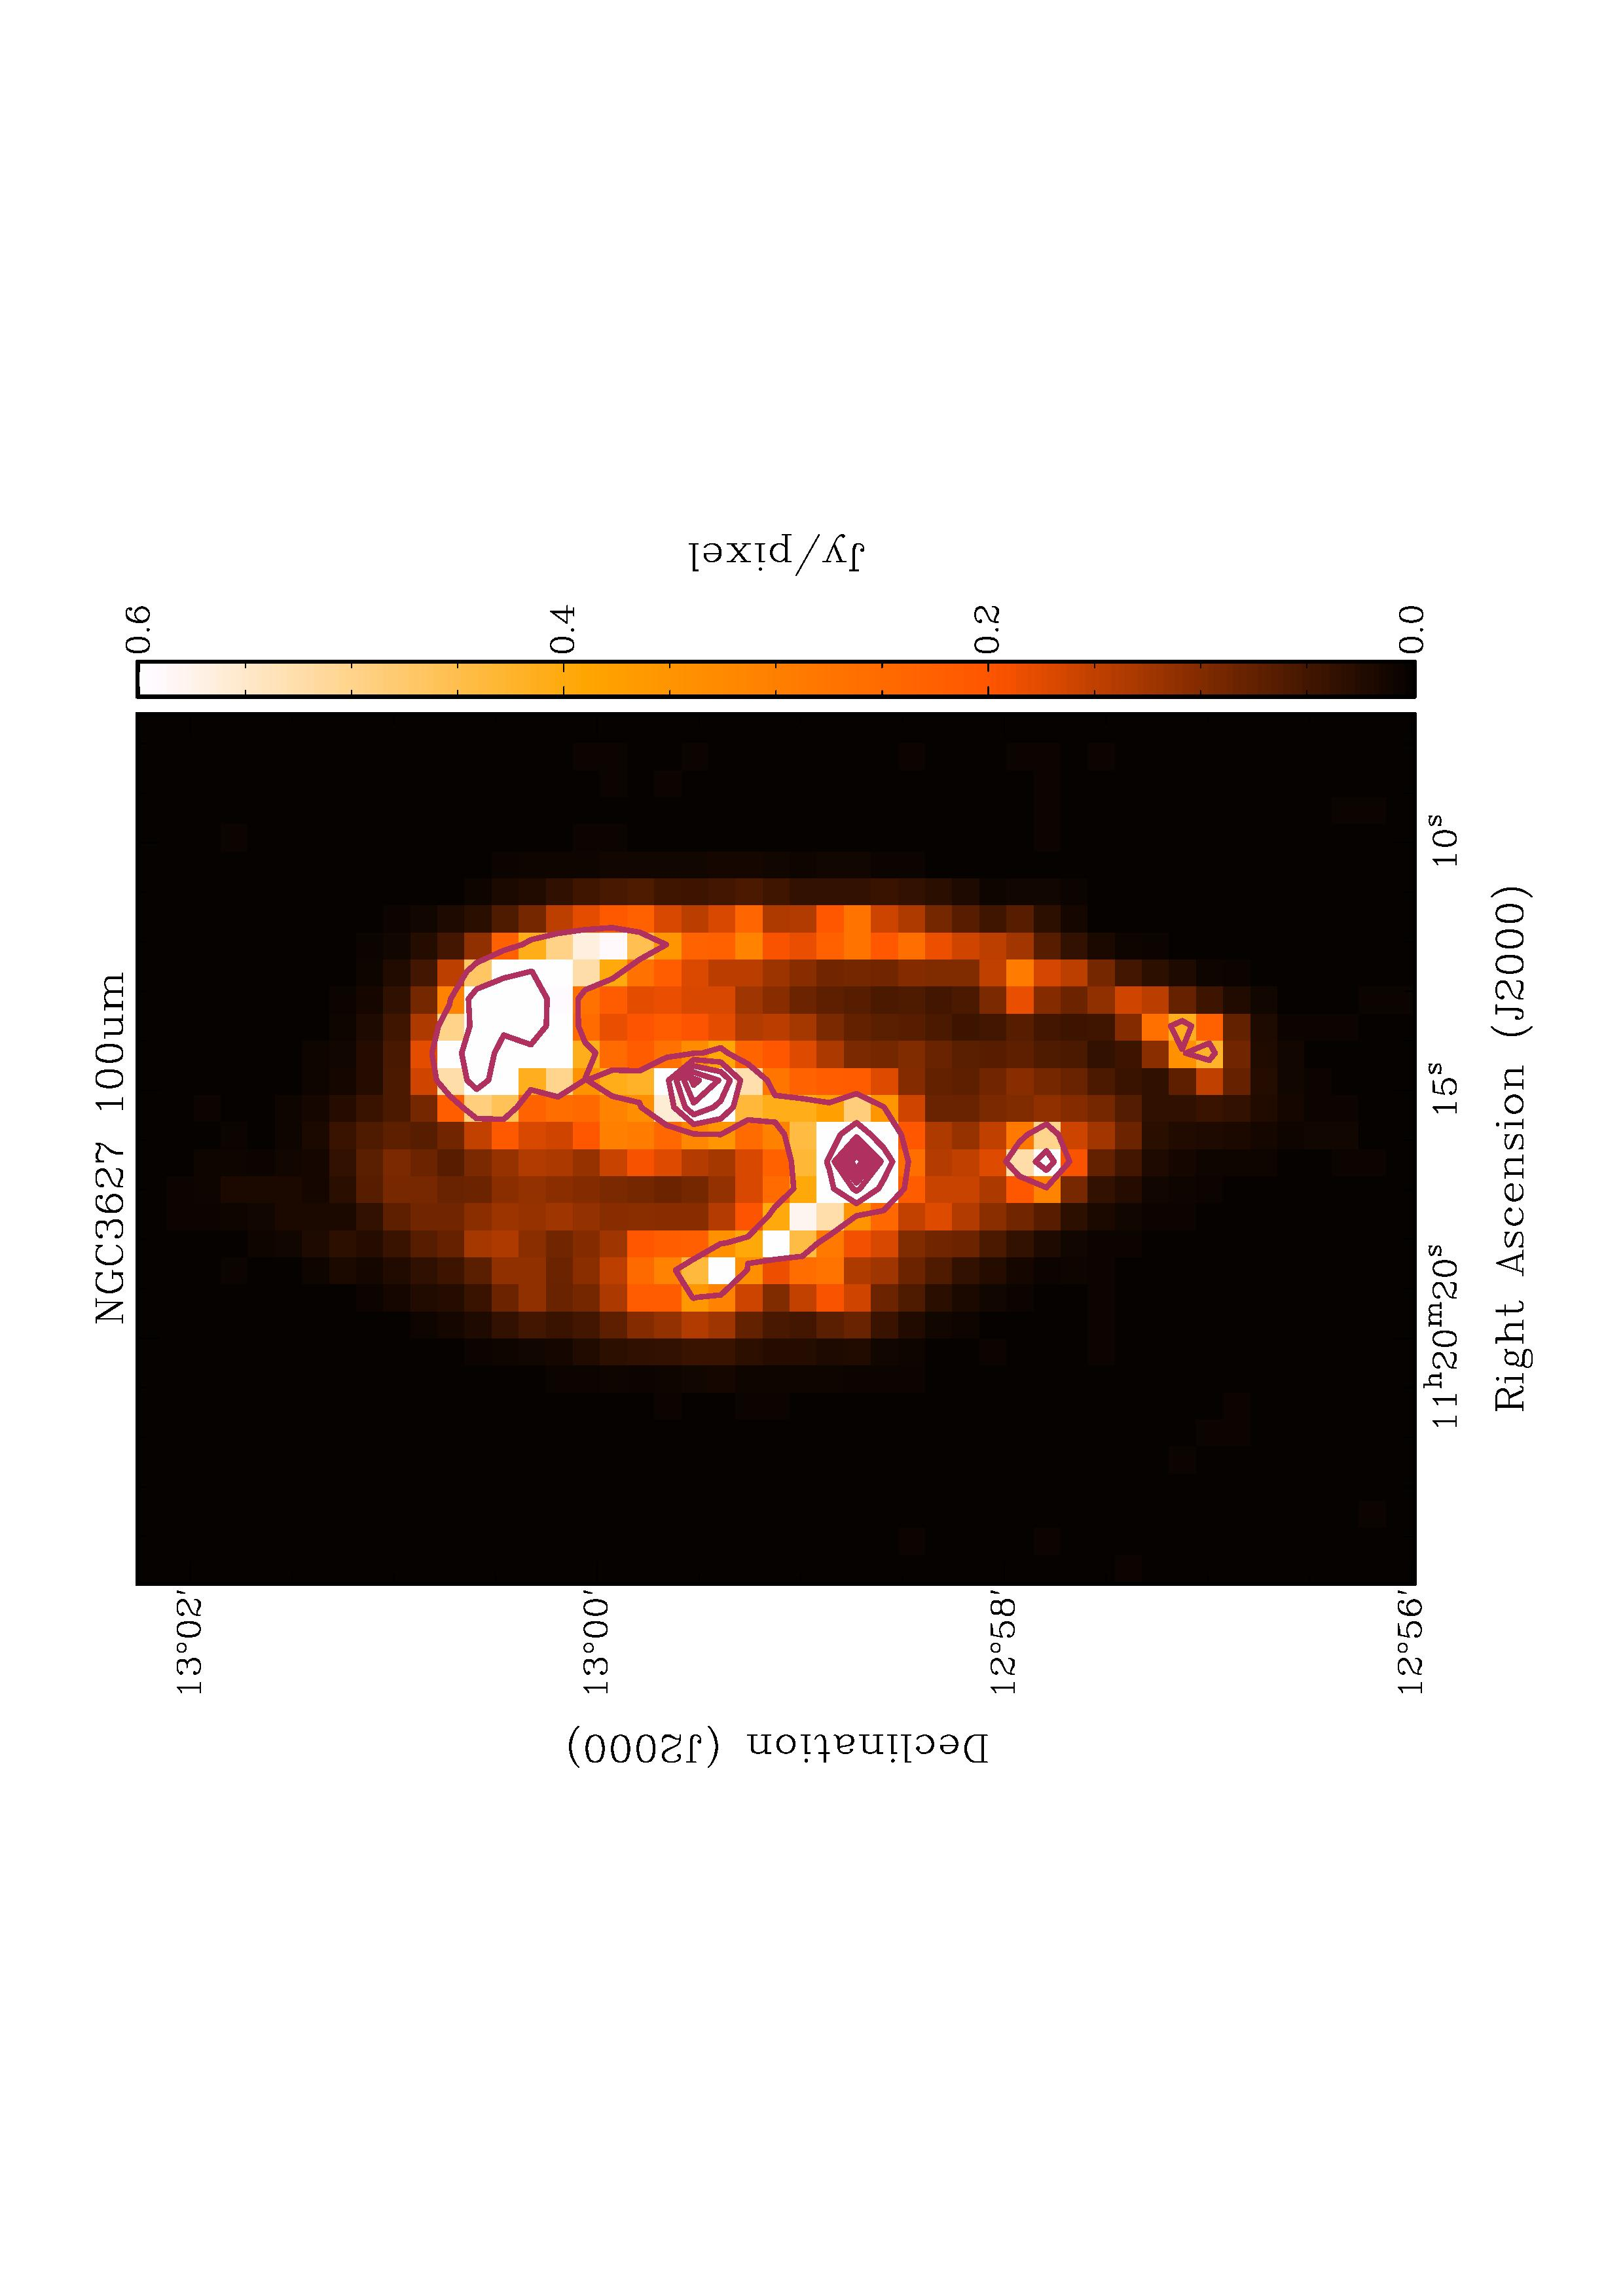
\includegraphics[scale=0.5,angle=270]{obs_imgs/100_um.jpeg}
  \caption[NGC3627 100$\mu$m Observations]{Residual of the MAKEMAP filtering of 100$\mu$m observations.}
\end{figure}

\begin{figure}
  \centering
  \label{fig_160}
  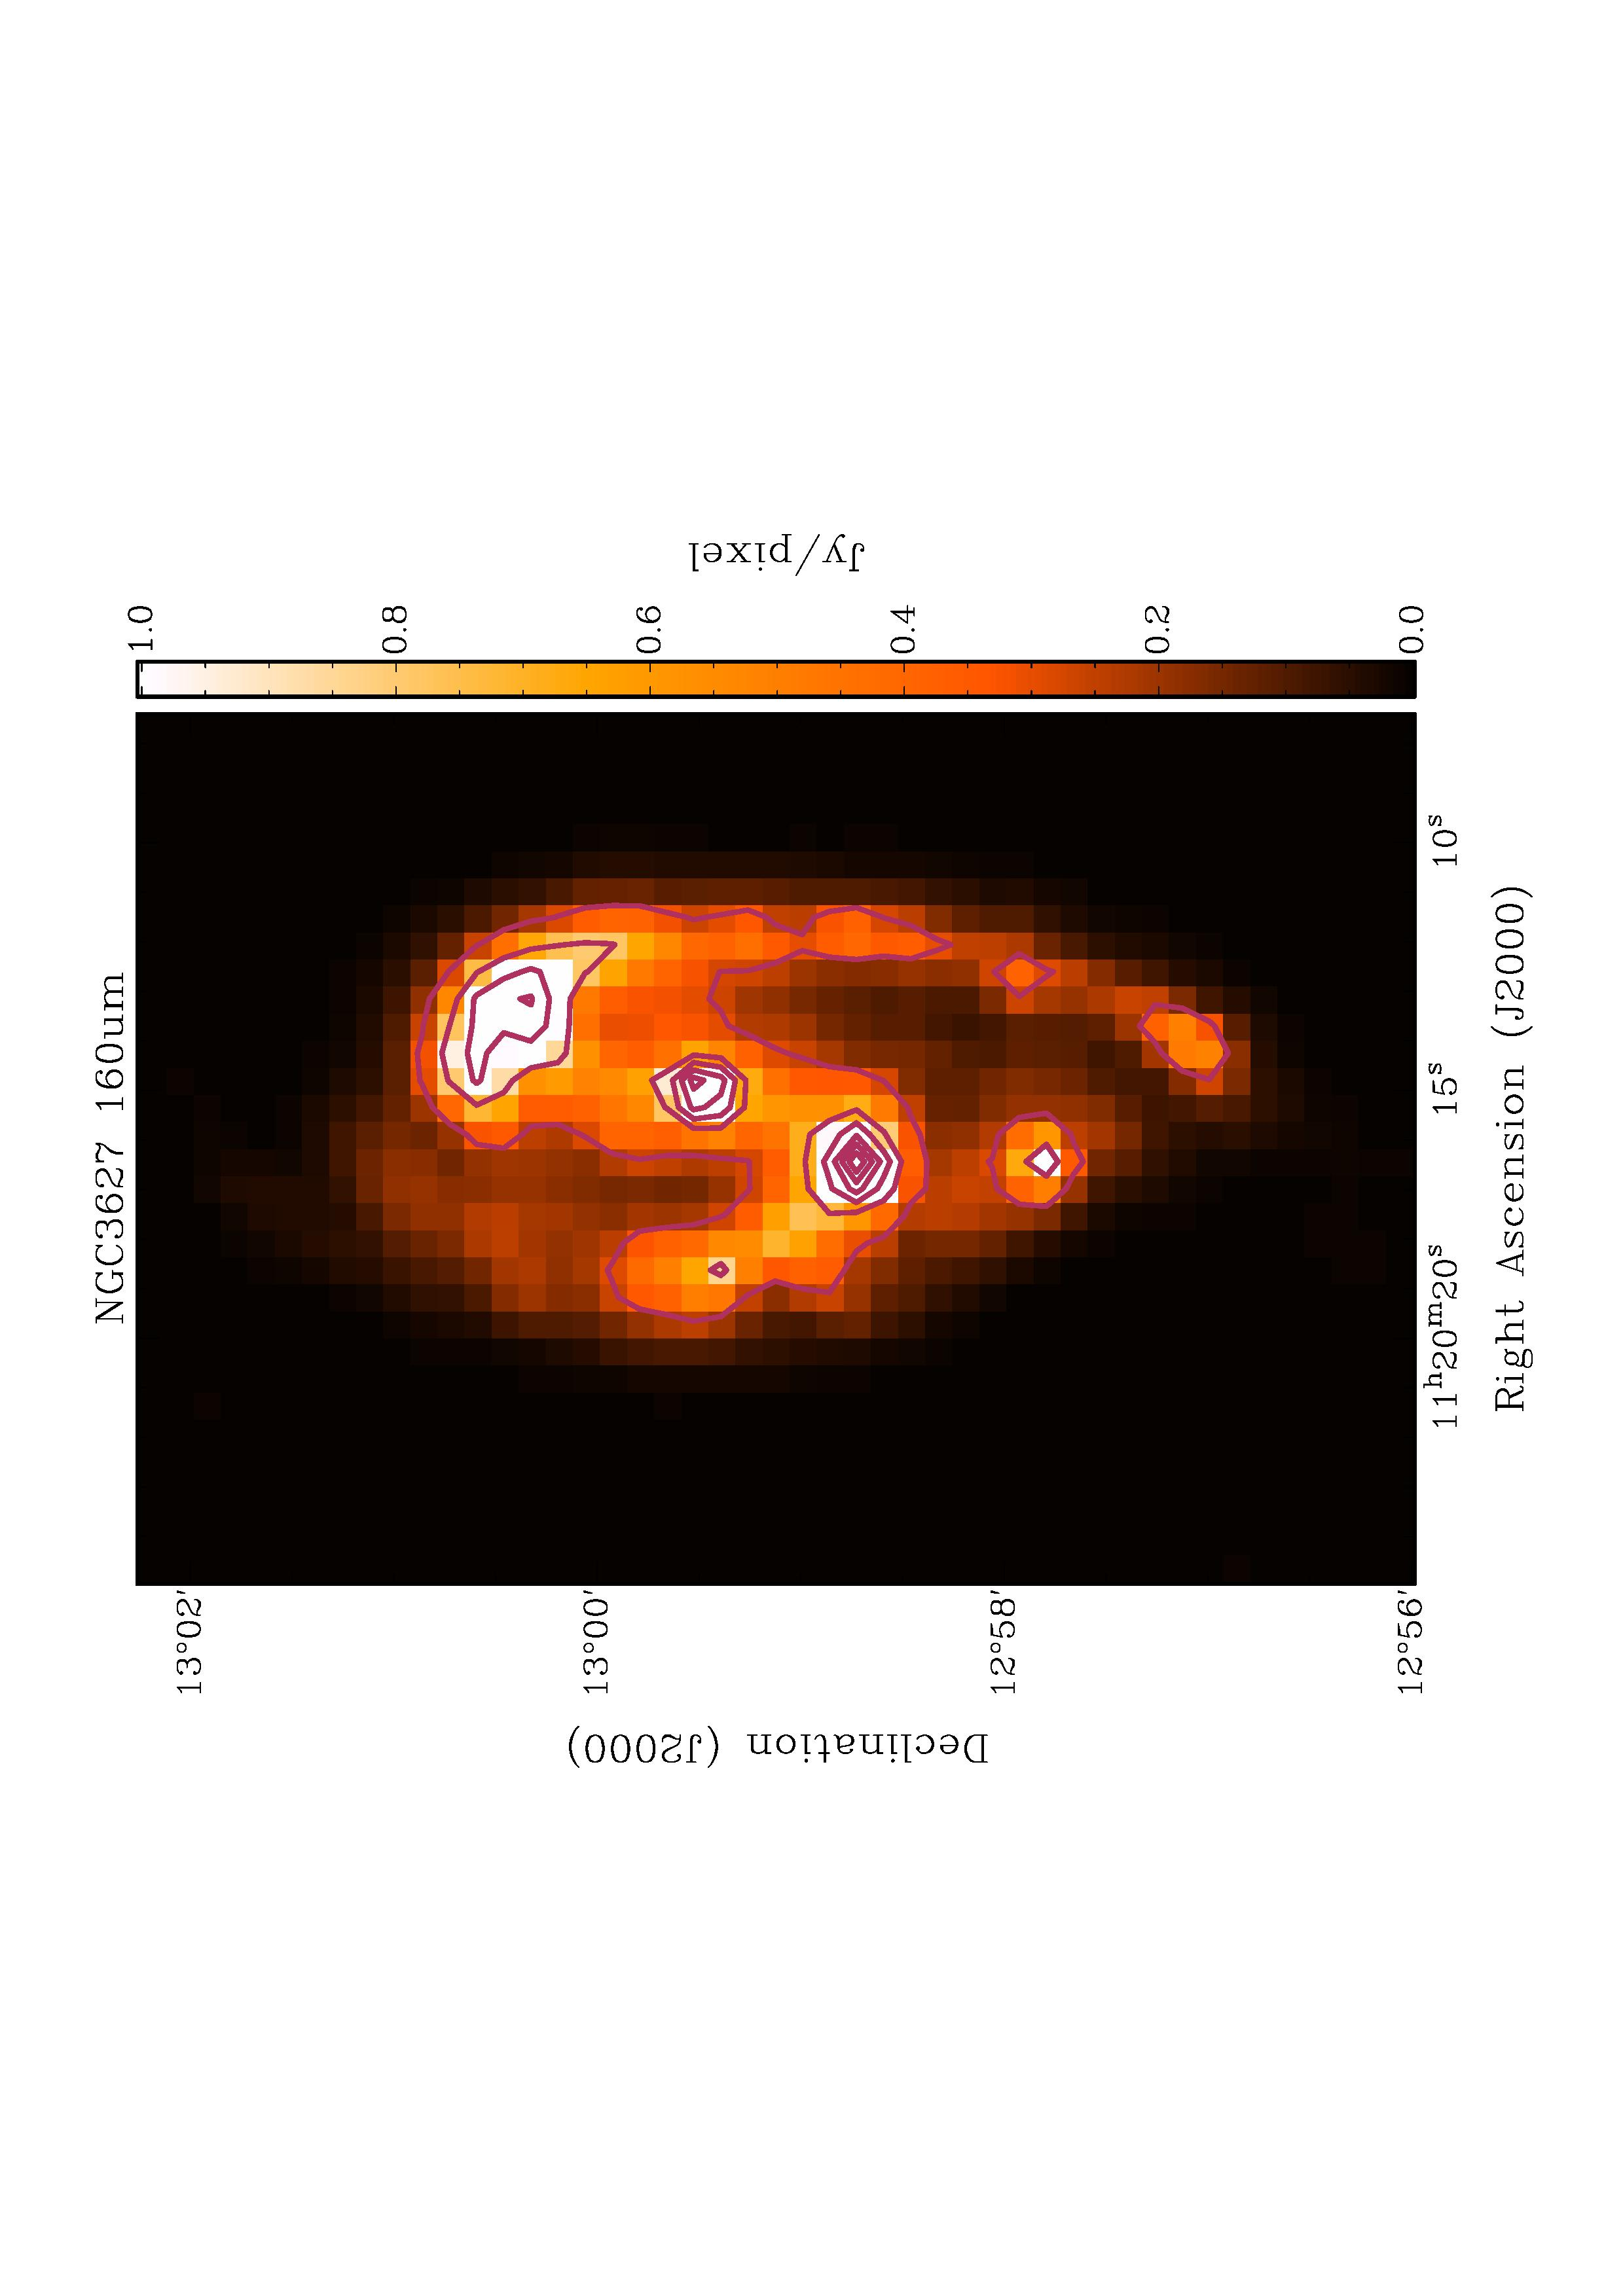
\includegraphics[scale=0.5,angle=270]{obs_imgs/160_um.jpeg}
  \caption[NGC3627 160$\mu$m Observations]{Residual of the MAKEMAP filtering of 160$\mu$m observations.}
\end{figure}

\begin{figure}
  \centering
  \label{fig_250}
  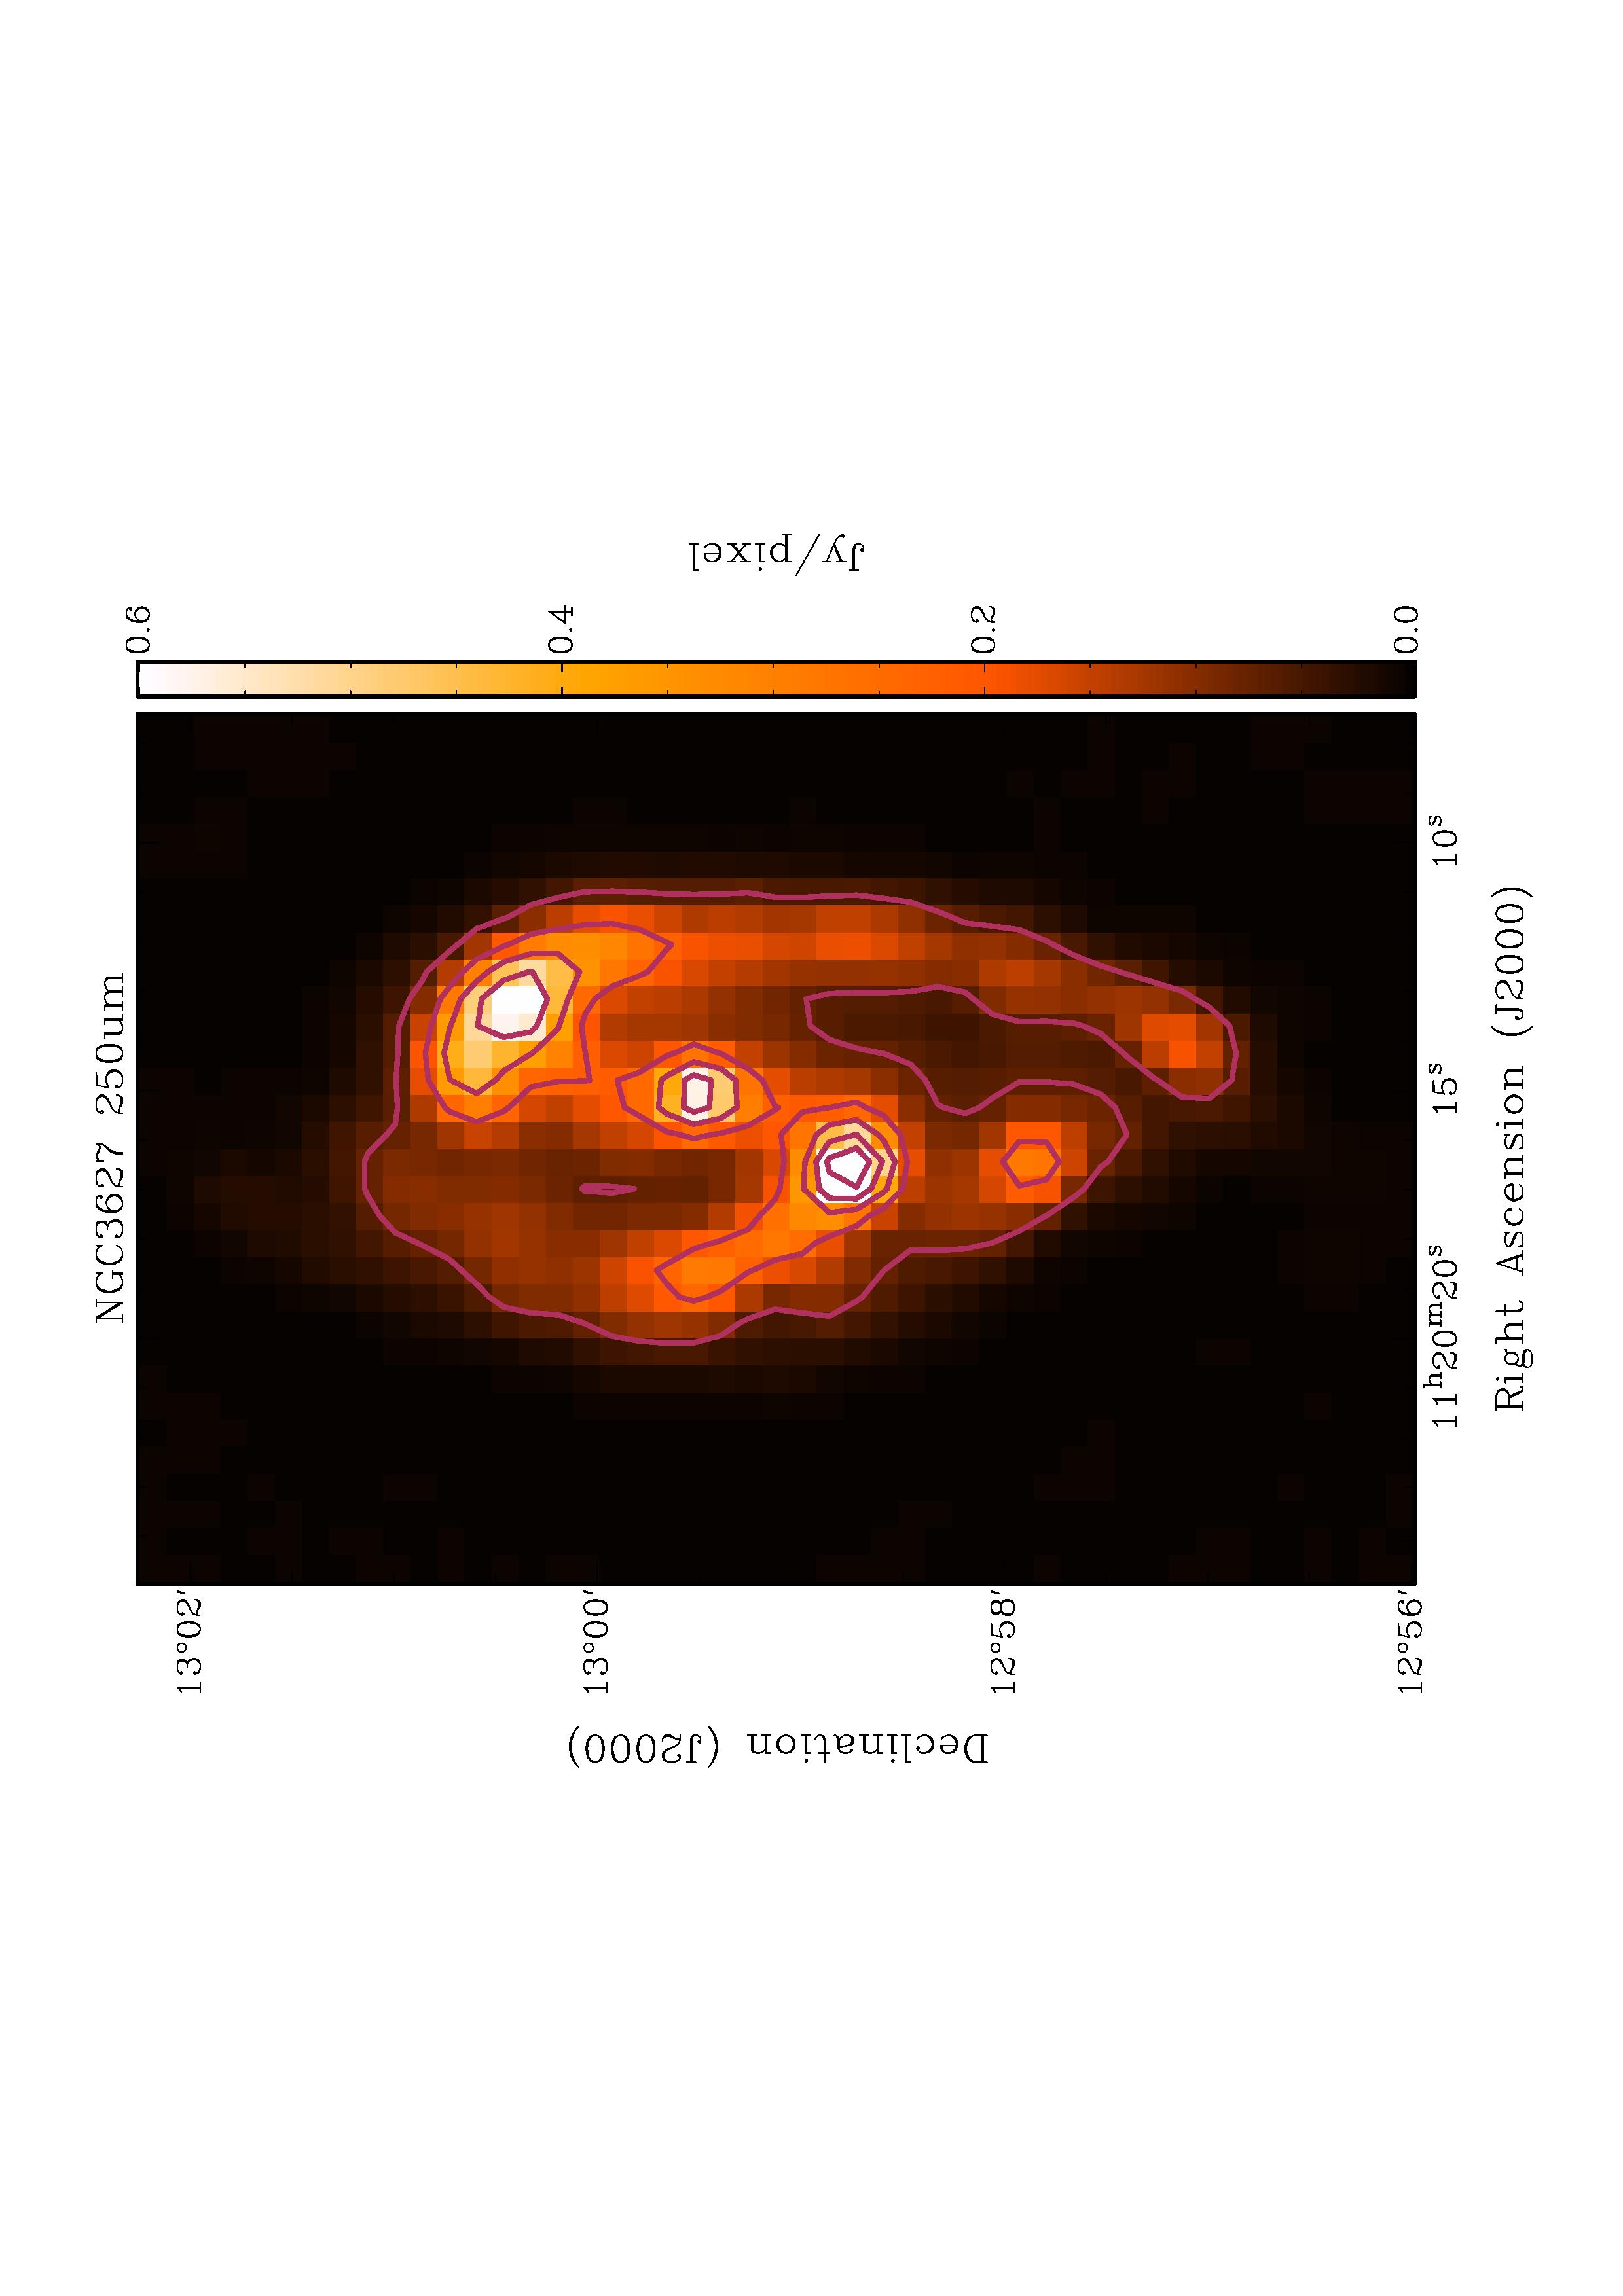
\includegraphics[scale=0.5,angle=270]{obs_imgs/250_um.jpeg}
  \caption[NGC3627 250$\mu$m Observations]{Residual of the MAKEMAP filtering of 250$\mu$m observations.}
\end{figure}

\begin{figure}
  \centering
  \label{fig_350}
  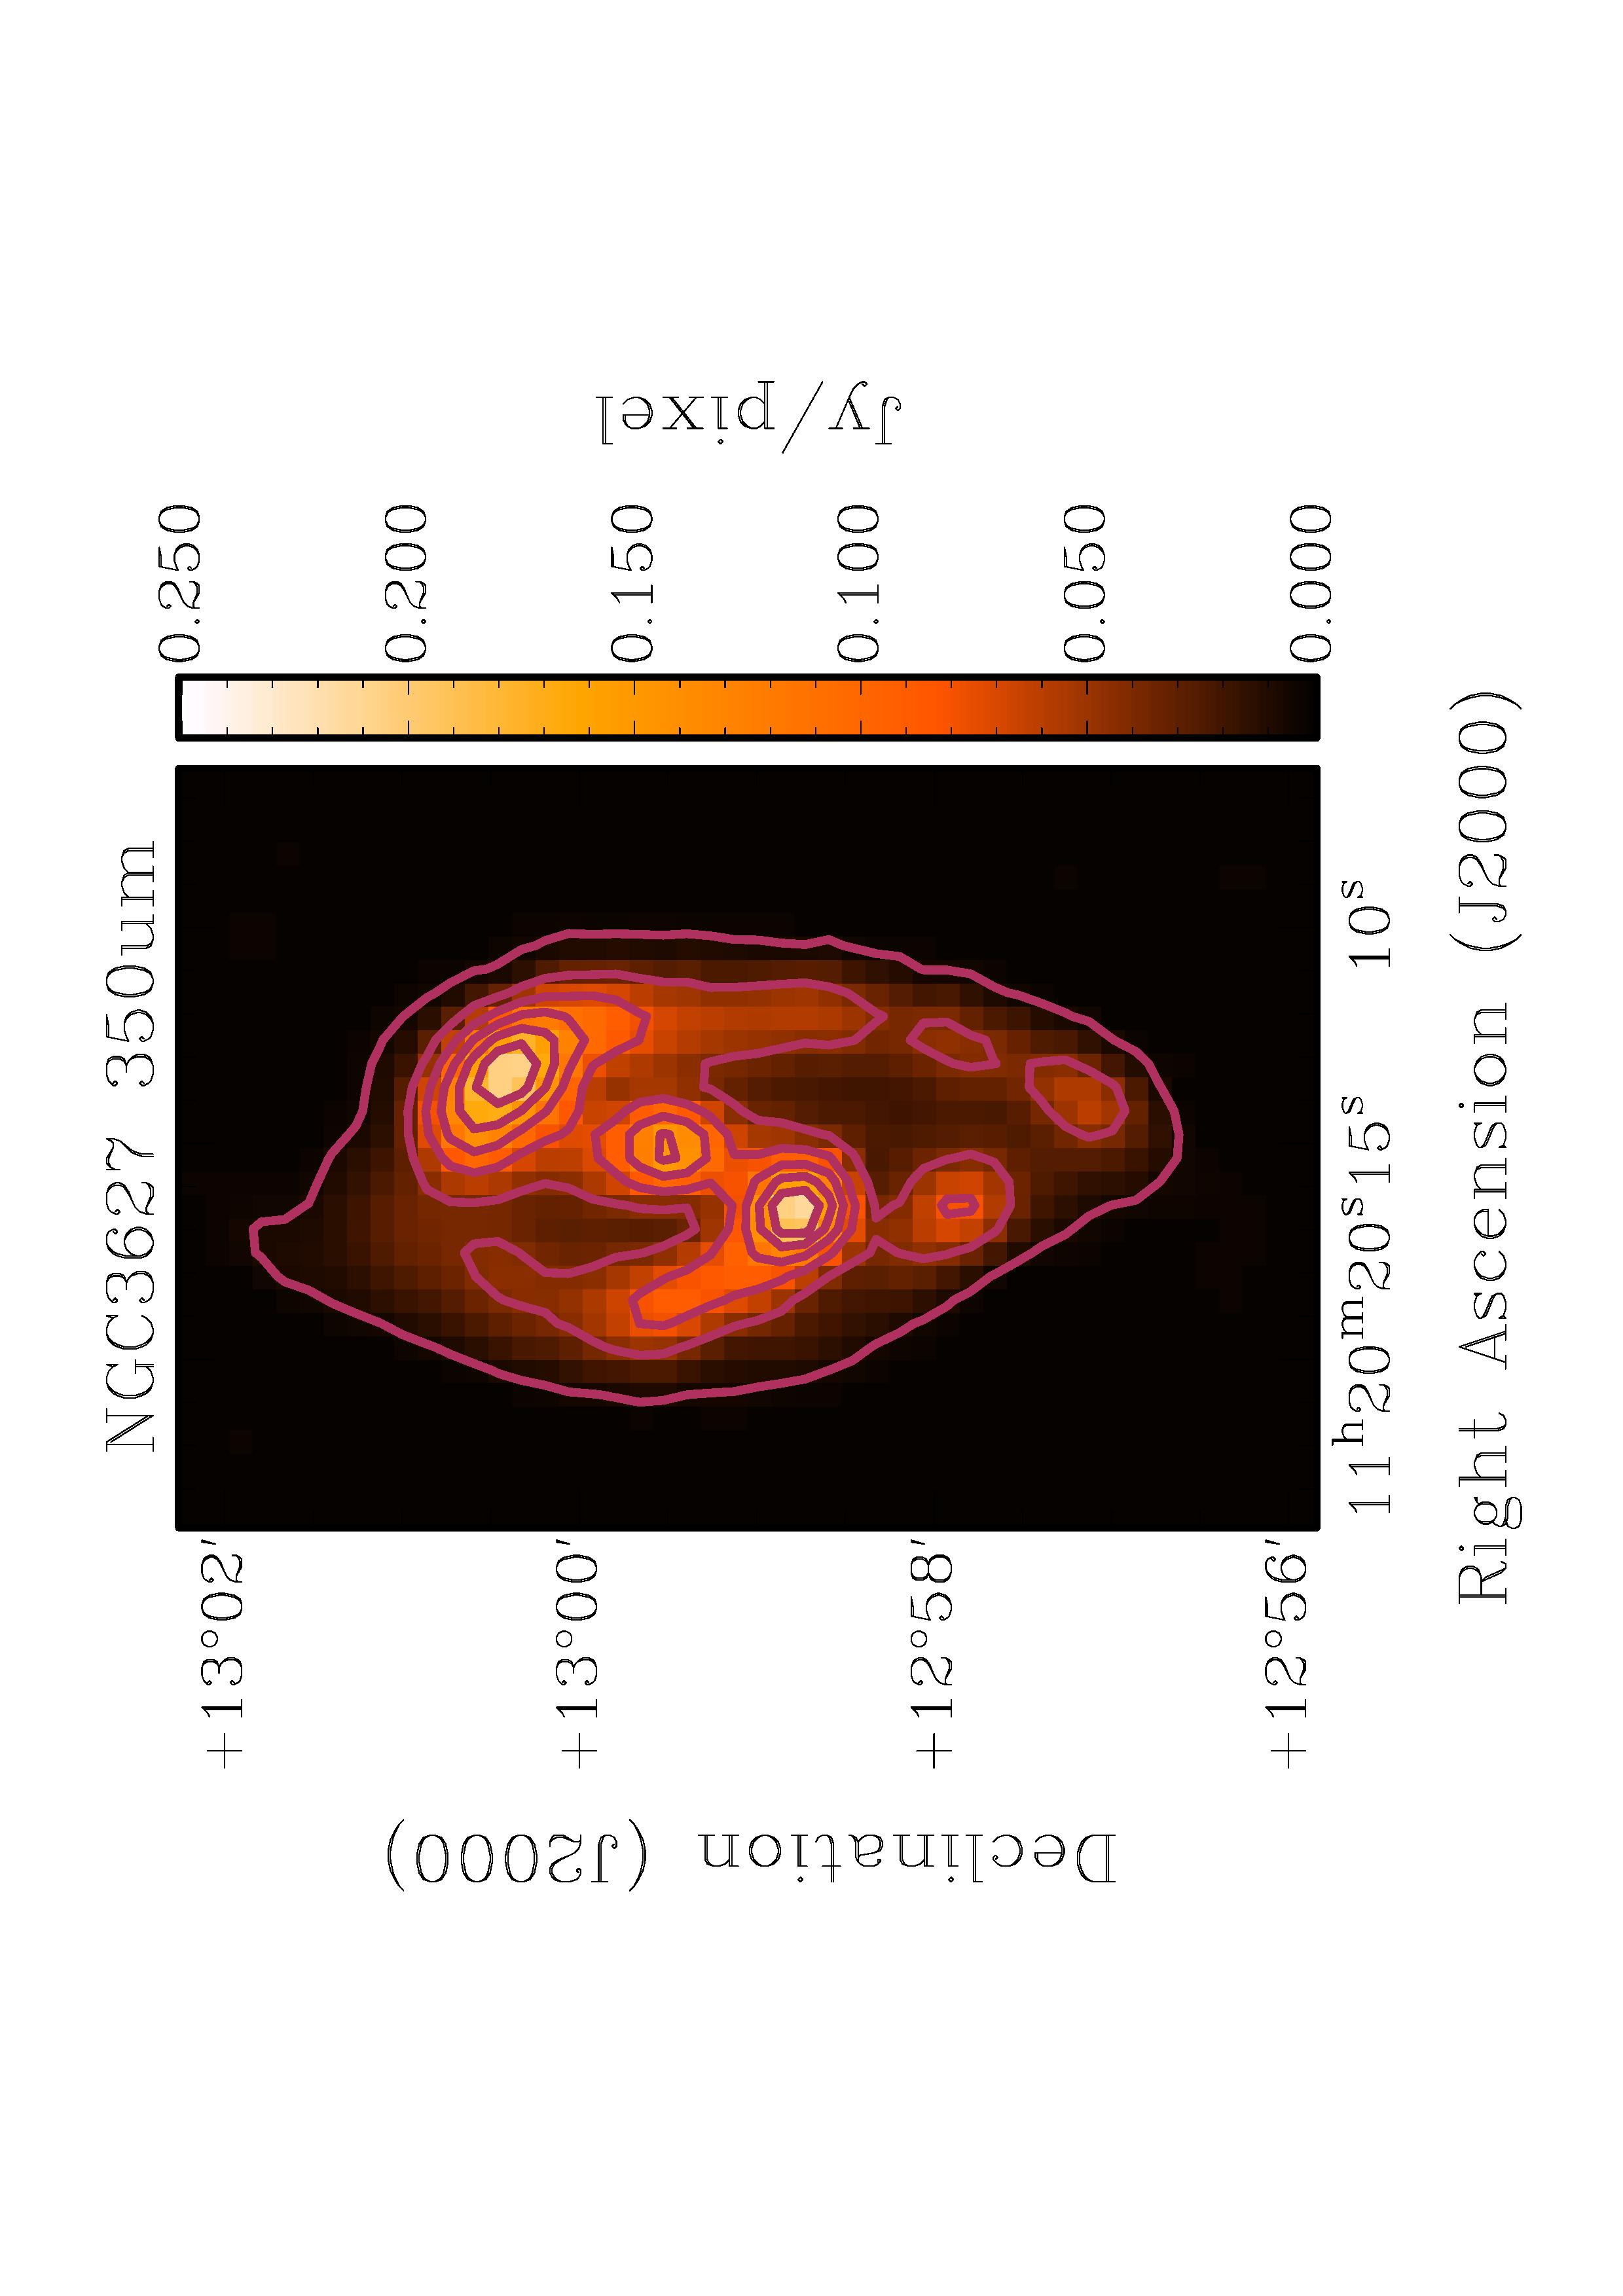
\includegraphics[scale=0.5,angle=270]{obs_imgs/350_um.jpeg}
  \caption[NGC3627 350$\mu$m Observations]{Residual of the MAKEMAP filtering of the 350$\mu$m observations.}
\end{figure}

\begin{figure}
  \centering
  \label{fig_500}
  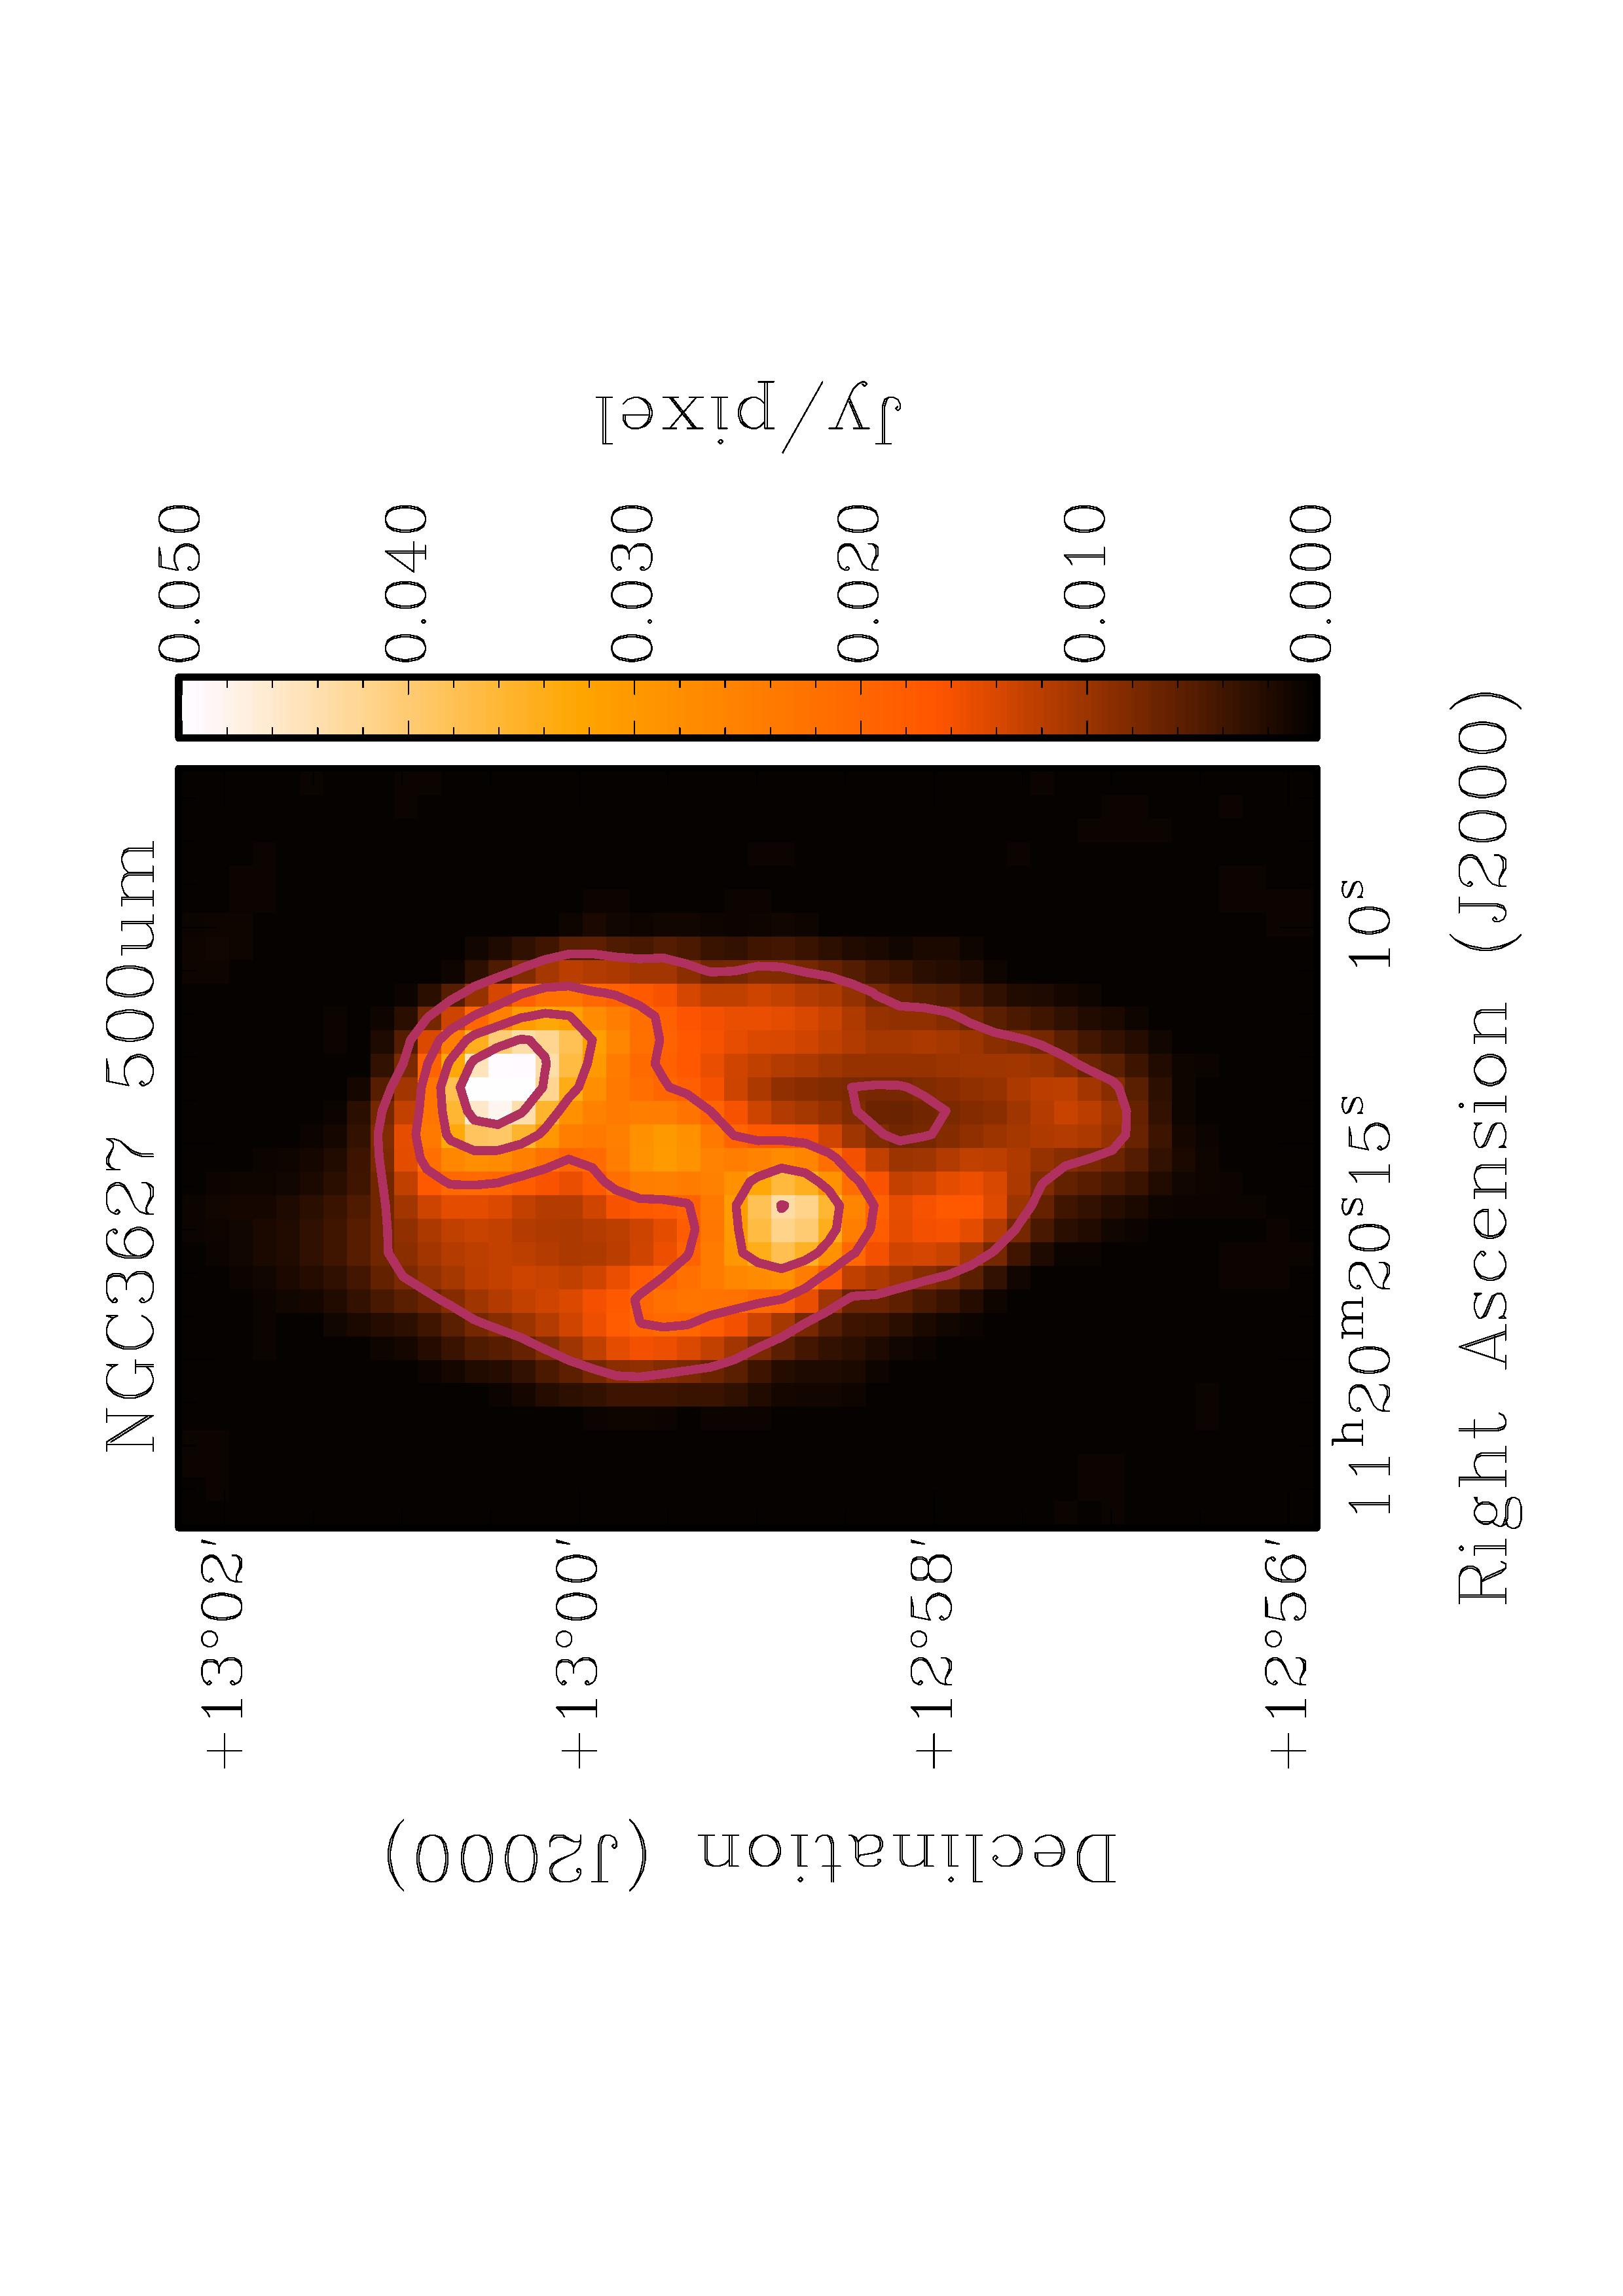
\includegraphics[scale=0.5,angle=270]{obs_imgs/500_um.jpeg}
  \caption[NGC3627 500$\mu$m Observations]{Residual of the MAKEMAP filtering of hte 500$\mu$m observations.}
\end{figure}

\begin{deluxetable}{cccc}
%  \tabletypesize{\footnotesize}
  \tablecolumns{4}
  \tablewidth{0pt}
  \tablecaption{Properties of NGC3627 KINGFISH Observations\label{tab_obs_kfish}}
  \tablehead{\colhead{Observation} & \colhead{Beam Properties } & \colhead{RMS} & \colhead{Percentage of Emission Removed} \\
 & $\theta_{beam}$ & \it{[Jy/Pixel]}}
  \startdata
    100$\mu$m & 6.8$\arcsec$ & 2.24e-3 & 16.7\% \\
    160$\mu$m & 11.6$\arcsec$ & 3.95e-3 & 18.8\% \\
    250$\mu$m & 18.0$\arcsec$ & 2.47e-3 & 19.9\% \\
    350$\mu$m & 24.9$\arcsec$ & 1.08e-3 & 21.8\% \\
    500$\mu$m & 36.0$\arcsec$ & 3.87e-4 & 27.7\% \\
  \enddata
\end{deluxetable}

\subsection{Nearby Galaxy Legacy Survey (NGLS)}

The Nearby Galaxy Legacy Survey is an HI-selected set of 155 galaxies contained in the annulus of $2Mpc\leq r \leq25Mpc$ using the instrumentation aboard the JCMT (\citet{wilson2012}).  The NGLS consists data observed in several wavelengths that include the 450$\mu$m and 850$\mu$m data used for this thesis.  As mentioned previously, the bandpass for SCUBA-2's 850$\mu$m emission contains the $CO_{j=3-2}$ line which is contained in the NGLS data set.  We used the zeroth moment $CO_{j=3-2}$ maps from the NGLS to determine the percentage of $CO_{j=3-2}$ emission present in the 850$\mu$m band as well as removing it for an accurate SED analysis.  

Removing the molecular gas contamination from the 850$\mu$m images required passing the data through MAKEMAP in a similar manner as the KINGFISH data.  The only significant difference was converting the $CO_{j=3-2}$ data from $K*km/s$ to pW.  The change of units was done using conversion factor of 0.70 $[K*km/s][mJy/beam]^{-1}$ found by \citet{drabek2012} for the task of converting HARP observations to the same units as SCUBA-2 850$\mu$m data.  The final image product can be seen in figure \ref{fig_co32}.  We found the average ratio of $CO_{j=3-2}$ to 850$\mu$m to be around 29\% with some regions dropping to less than 6\%.  The amount of flux removed and the filtered image's rms can be found in table \ref{tab_obs_NGLS}.

\begin{figure}
  \centering
  \label{fig_co32}
  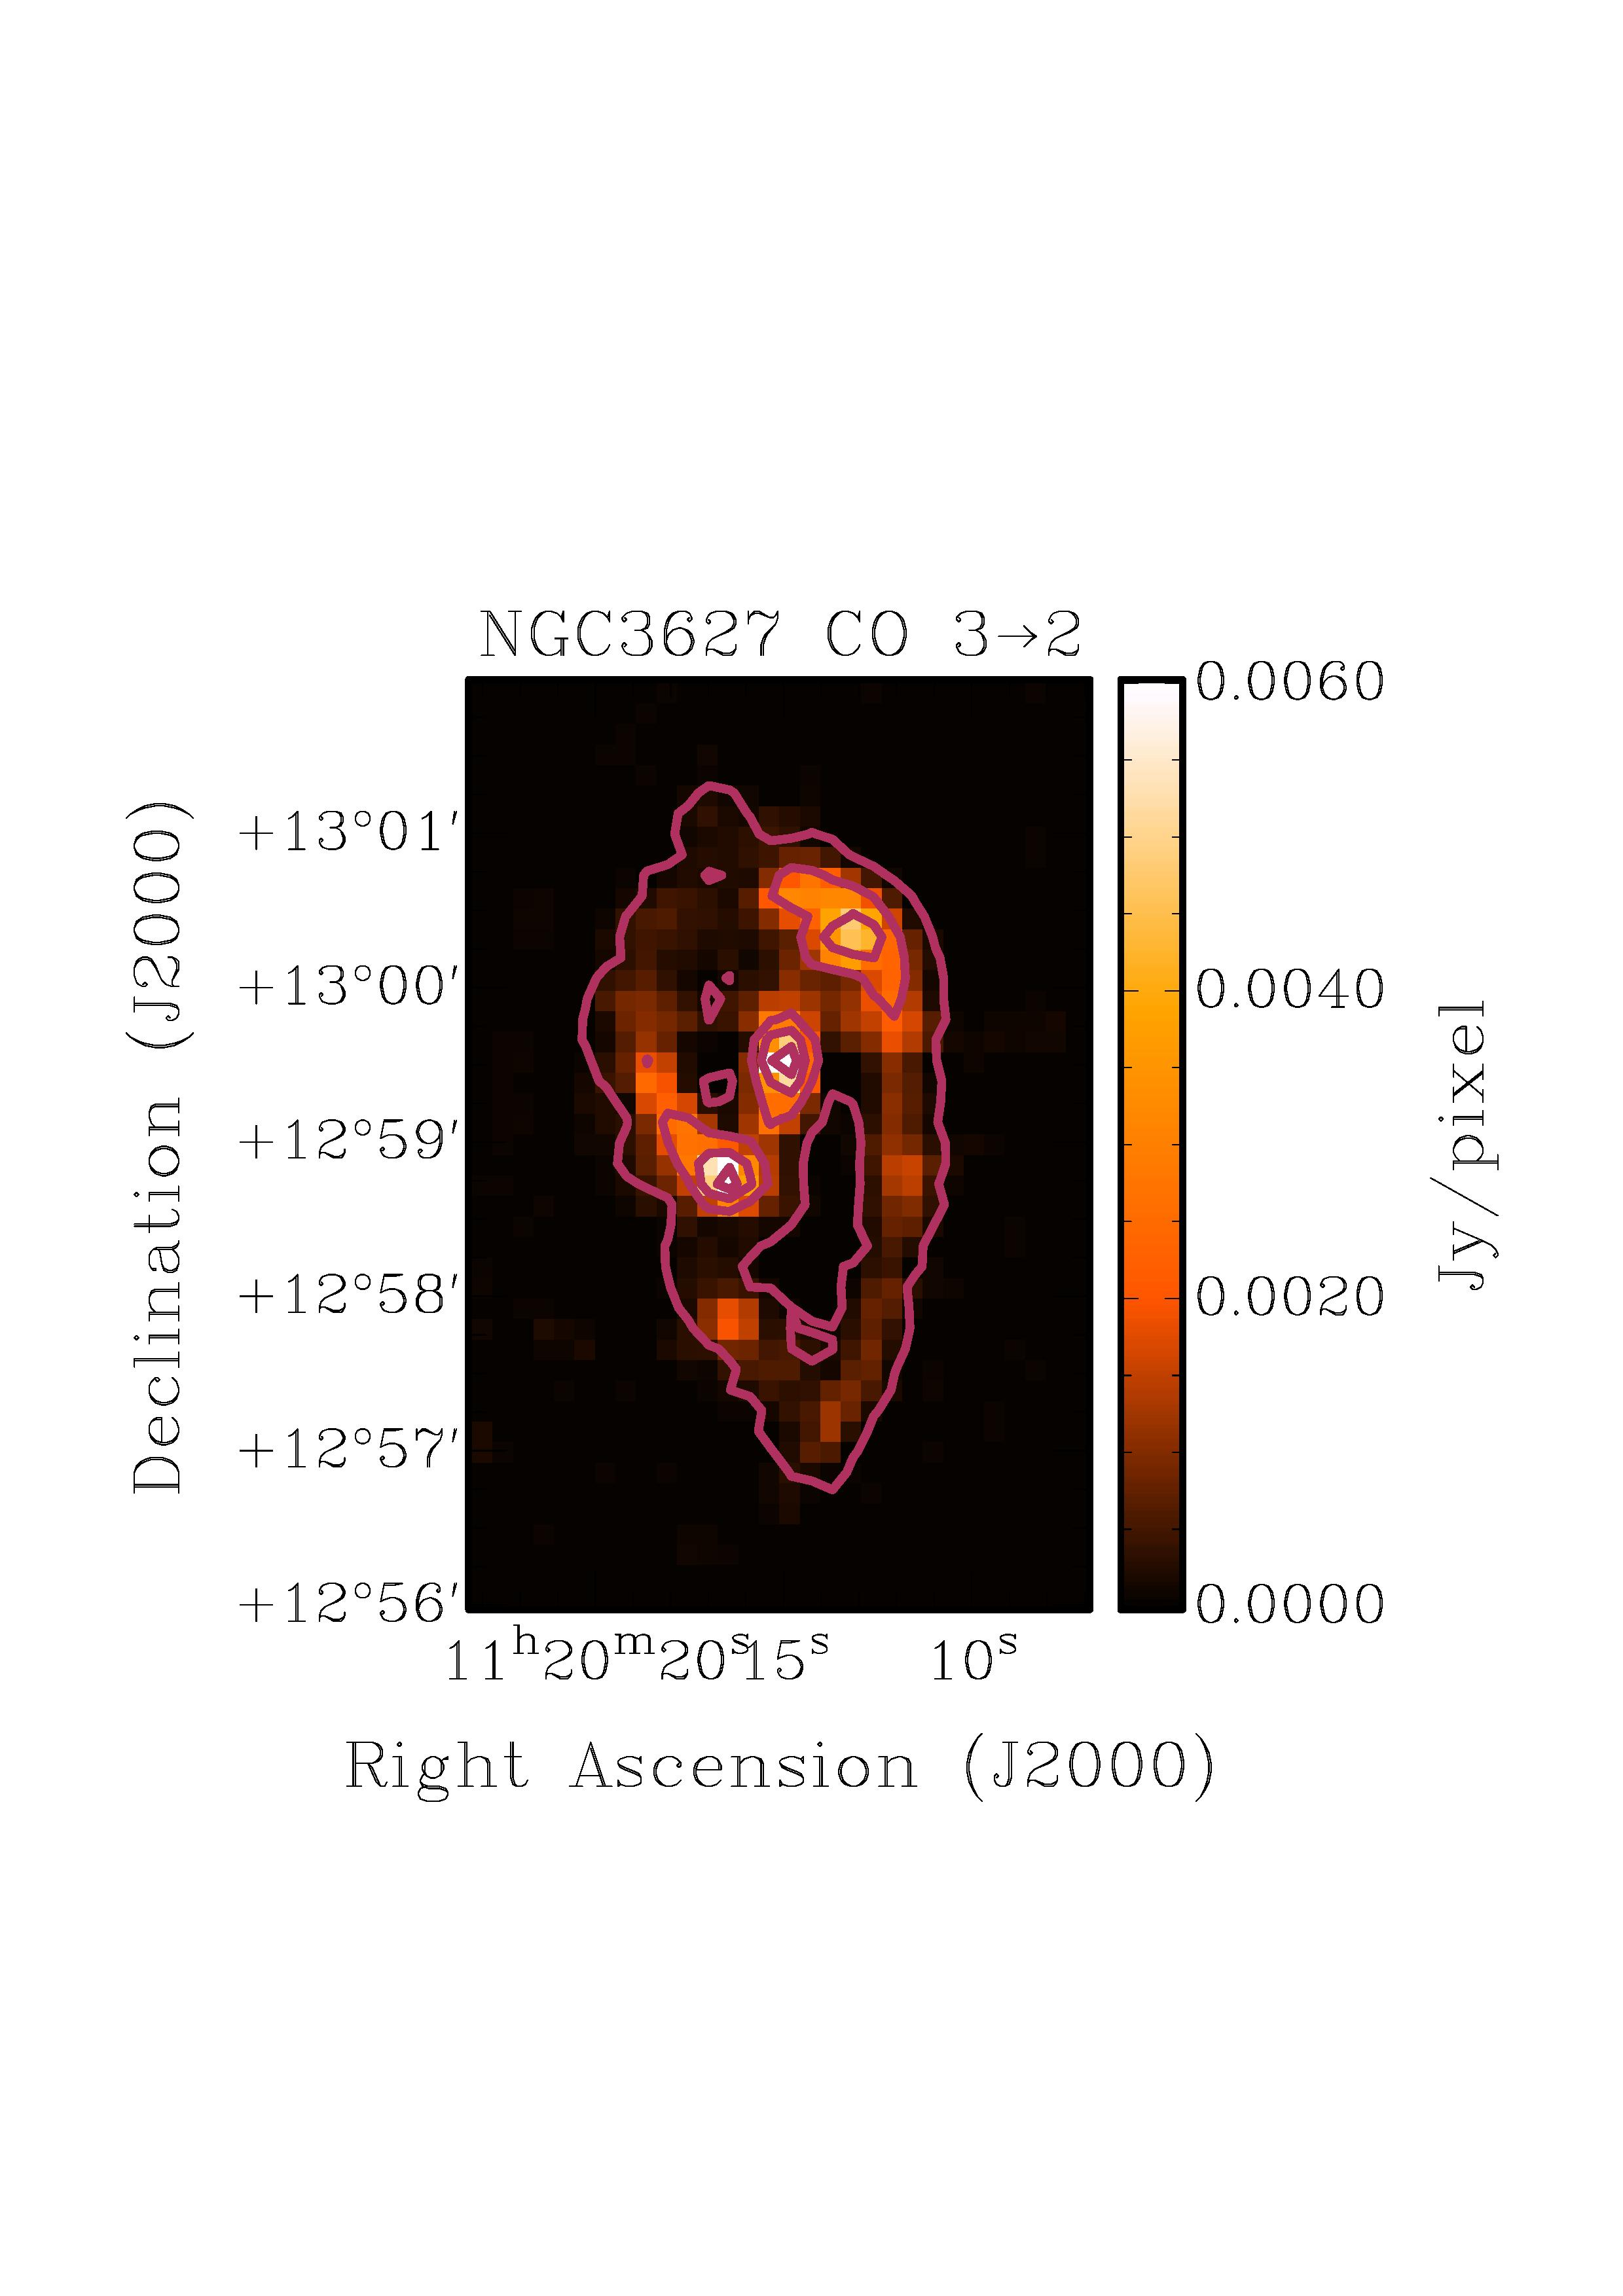
\includegraphics[scale=0.5]{obs_imgs/CO32.jpeg}
  \caption[NGC3627 $CO_{j=3-2}$ Observations]{Residual of the MAKEMAP filtering of $CO_{j=3-2}$ observations.}
\end{figure}

\begin{deluxetable}{cccc}
  \tablecolumns{4}
  \tablewidth{0pt}
  \tablecaption{Properties of NGC3627 NGLS Observations\label{tab_obs_NGLS}}
  \tablehead{\colhead{Observation} & \colhead{Beam Properties } & \colhead{RMS} & \colhead{Percentage of Emission Removed} \\
 & $\theta_{beam}$ & \it{[Jy/Pixel]}}
  \startdata
    $CO_{j=3-2}$ & 14.5$\arcsec$ & 1.28e-5& 29.8\% \\
  \enddata
\end{deluxetable}

%insert co32 img

\subsection{Nobeyama 45-m}\label{nob_sec}

Determining a dust-to-gas ratio required the need for a molecular tracer to estimate the amount of molecular hydrogen present.  The most frequently used tracer is $CO_{j=1-0}$ due to its abundance in the ISM.  The $CO_{j=1-0}$ we used was taken from the Nobeyama 45-m CO Atlas of Nearby Spiral Galaxies and observed to better understand the roll of bars relating to molecular gas (\citet{kuno2007}).  The Nobeyama 45-m CO Atlas consists of galaxies with morphologies ranging from Sa to Scd, located less that 25Mpc from the Milky Way, inclination values greater that $79^{\circ}$, 100$\mu$m flux greater than 10Jy, and spiral structure that has not be comprimised through interactions.  Any galaxies that met this criteria were then observed with the Nobeyama 45-m telescope (\citet{kuno2007})

Preparation for the $CO_{j=1-0}$ was performed in a similar matter to the previous ancillary data sets, however instead of determining a direct conversion factor the zeroth moment map was scaled down by a factor 0.001.  The scaling factor used was used in lieu of the unit conversion method so the final image would be in it's native units of ($K km/s$) at the end of filtering.  The scaling factor was determined in a way such that the input image for the fakesoure would be on the same order of magnitude as the 850$\mu$m image it was being added onto.  The scaling factor was then re-applied as the flux calibration factor to return the filtered map to its original magnitude.  The beam sizes and rms of the filterd $CO_{j=1-0}$ map are displayed in table \ref{tab_obs_n45} and the final image product can be seen in figure \ref{fig_co10}.

\begin{figure}
  \centering
  \label{fig_co10}
  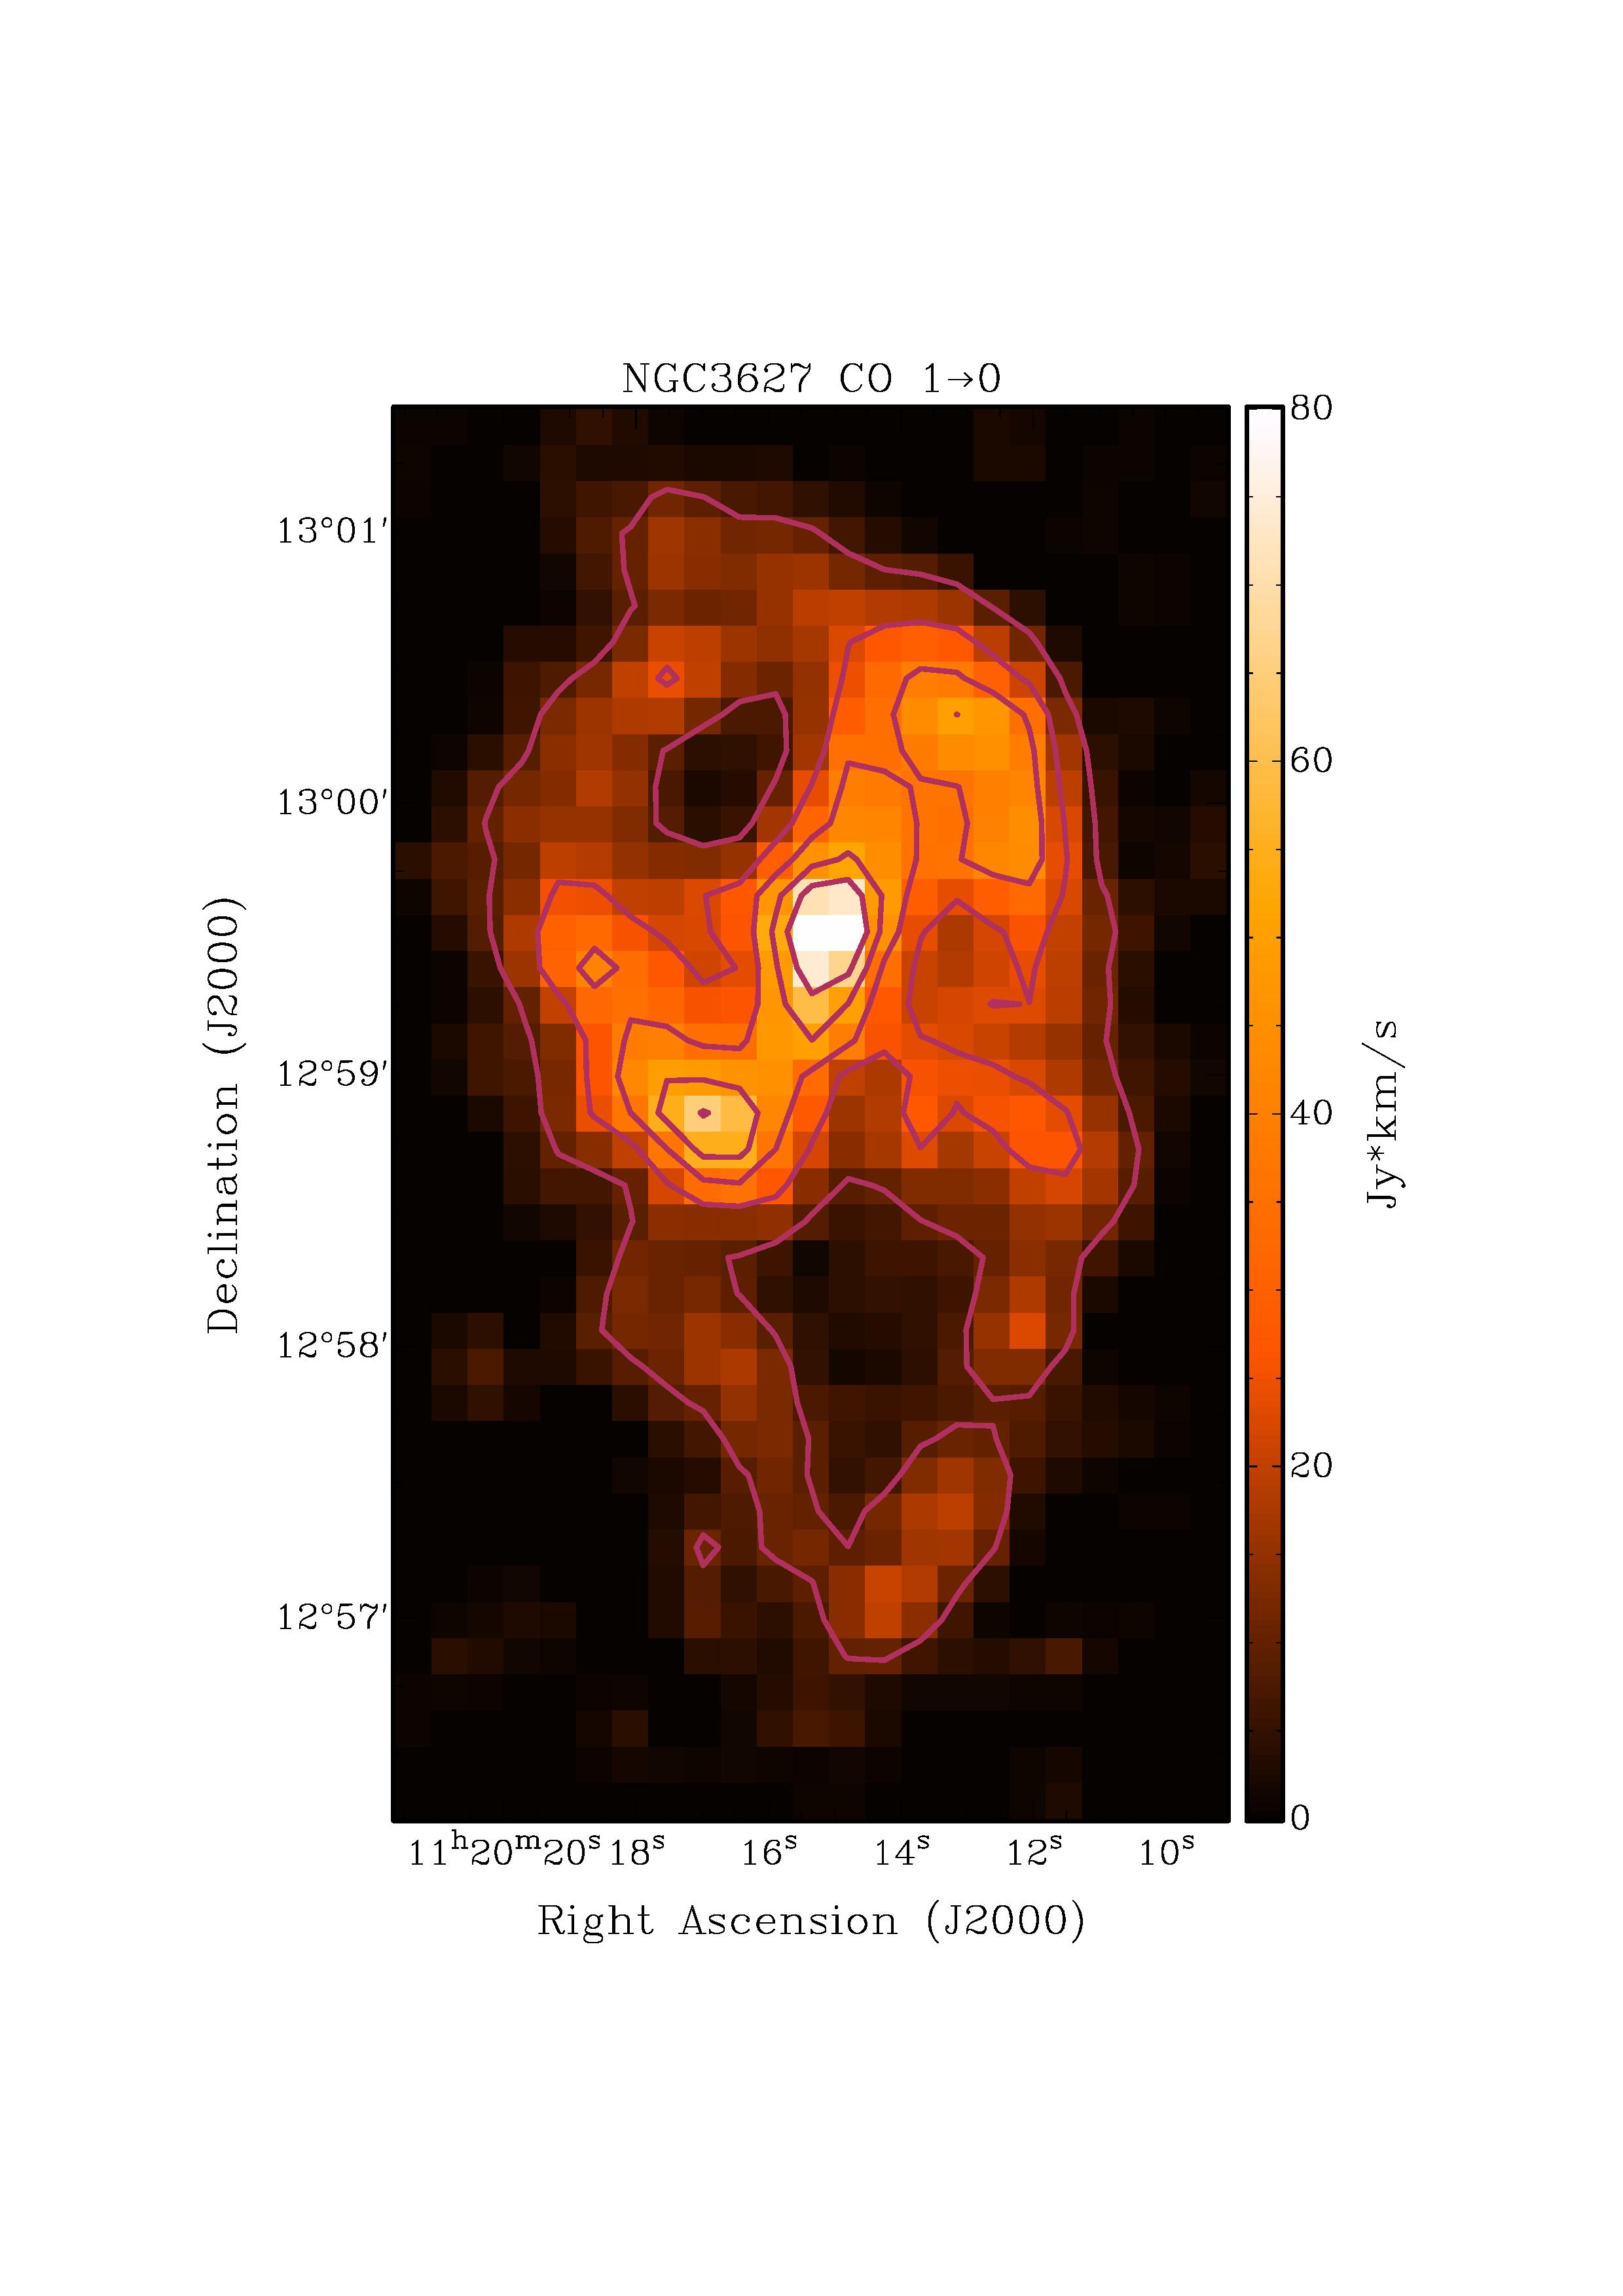
\includegraphics[scale=0.5]{obs_imgs/CO10.jpeg}
  \caption[NGC3627 $CO_{j=1-0}$ Observations]{Residual of the MAKEMAP filtering of $CO_{j=1-0}$ observations.}
\end{figure}

\begin{deluxetable}{cccc}
  \tablecolumns{4}
  \tablewidth{0pt}
  \tablecaption{Properties of NGC3627 Nobeyama 45-m Observations\label{tab_obs_n45}}
  \tablehead{\colhead{Observation} & \colhead{Beam Properties } & \colhead{RMS} & \colhead{Percentage of Emission Removed} \\ 
  & $\theta_{beam}$ & \it{[K km/s]}}
  \startdata
    $CO_{j=1-0}$ & 15.0$\arcsec$ & 0.681 & 25.8\% \\
  \enddata
\end{deluxetable}

\subsection{Hetrodyne Reciever Array CO-Line Extragalactic Survey (HERACLES)}

The $CO_{j=2-1}$ line was used to determine a ${2-1} / {1-0}$ line ratio which can be used to trace a gradient in $\alpha_{CO}$ and hint towards regions of high star-formation \citet{reuter1996}.  We used the $CO_{j=1-0}$ data from the Nobeyama 45-m telescope ($\S$ \ref{nob_sec}), and $CO_{j=2-1}$ from the Hetrodyne Reciever Array CO-Line Extragalactic Survey (HERACLES) using the IRAM 30-m telescope.  The main goal of HERACLES was to quantify the relationship between atomic and molecular gas and star formation using a large sample of galaxies (\citet{leroy2009}).  The sample of galaxies chosen were targets contained in THINGS that were within observing limits of the IRAM 30-m telescope.

The HERACLES data was treated in the same manner as the Nobeyama 45-m when filtering was applied.  Since both the $CO_{j=1-0}$ and $CO_{j=2-1}$ were on the same order of magnitude, the same scaling factor of 0.001 was applied before and after the filtering.  The final image can be seen in figure \ref{fig_co21} and the image properties can be seen in table \ref{tab_obs_heracles}.

\begin{figure}
  \centering
  \label{fig_co21}
  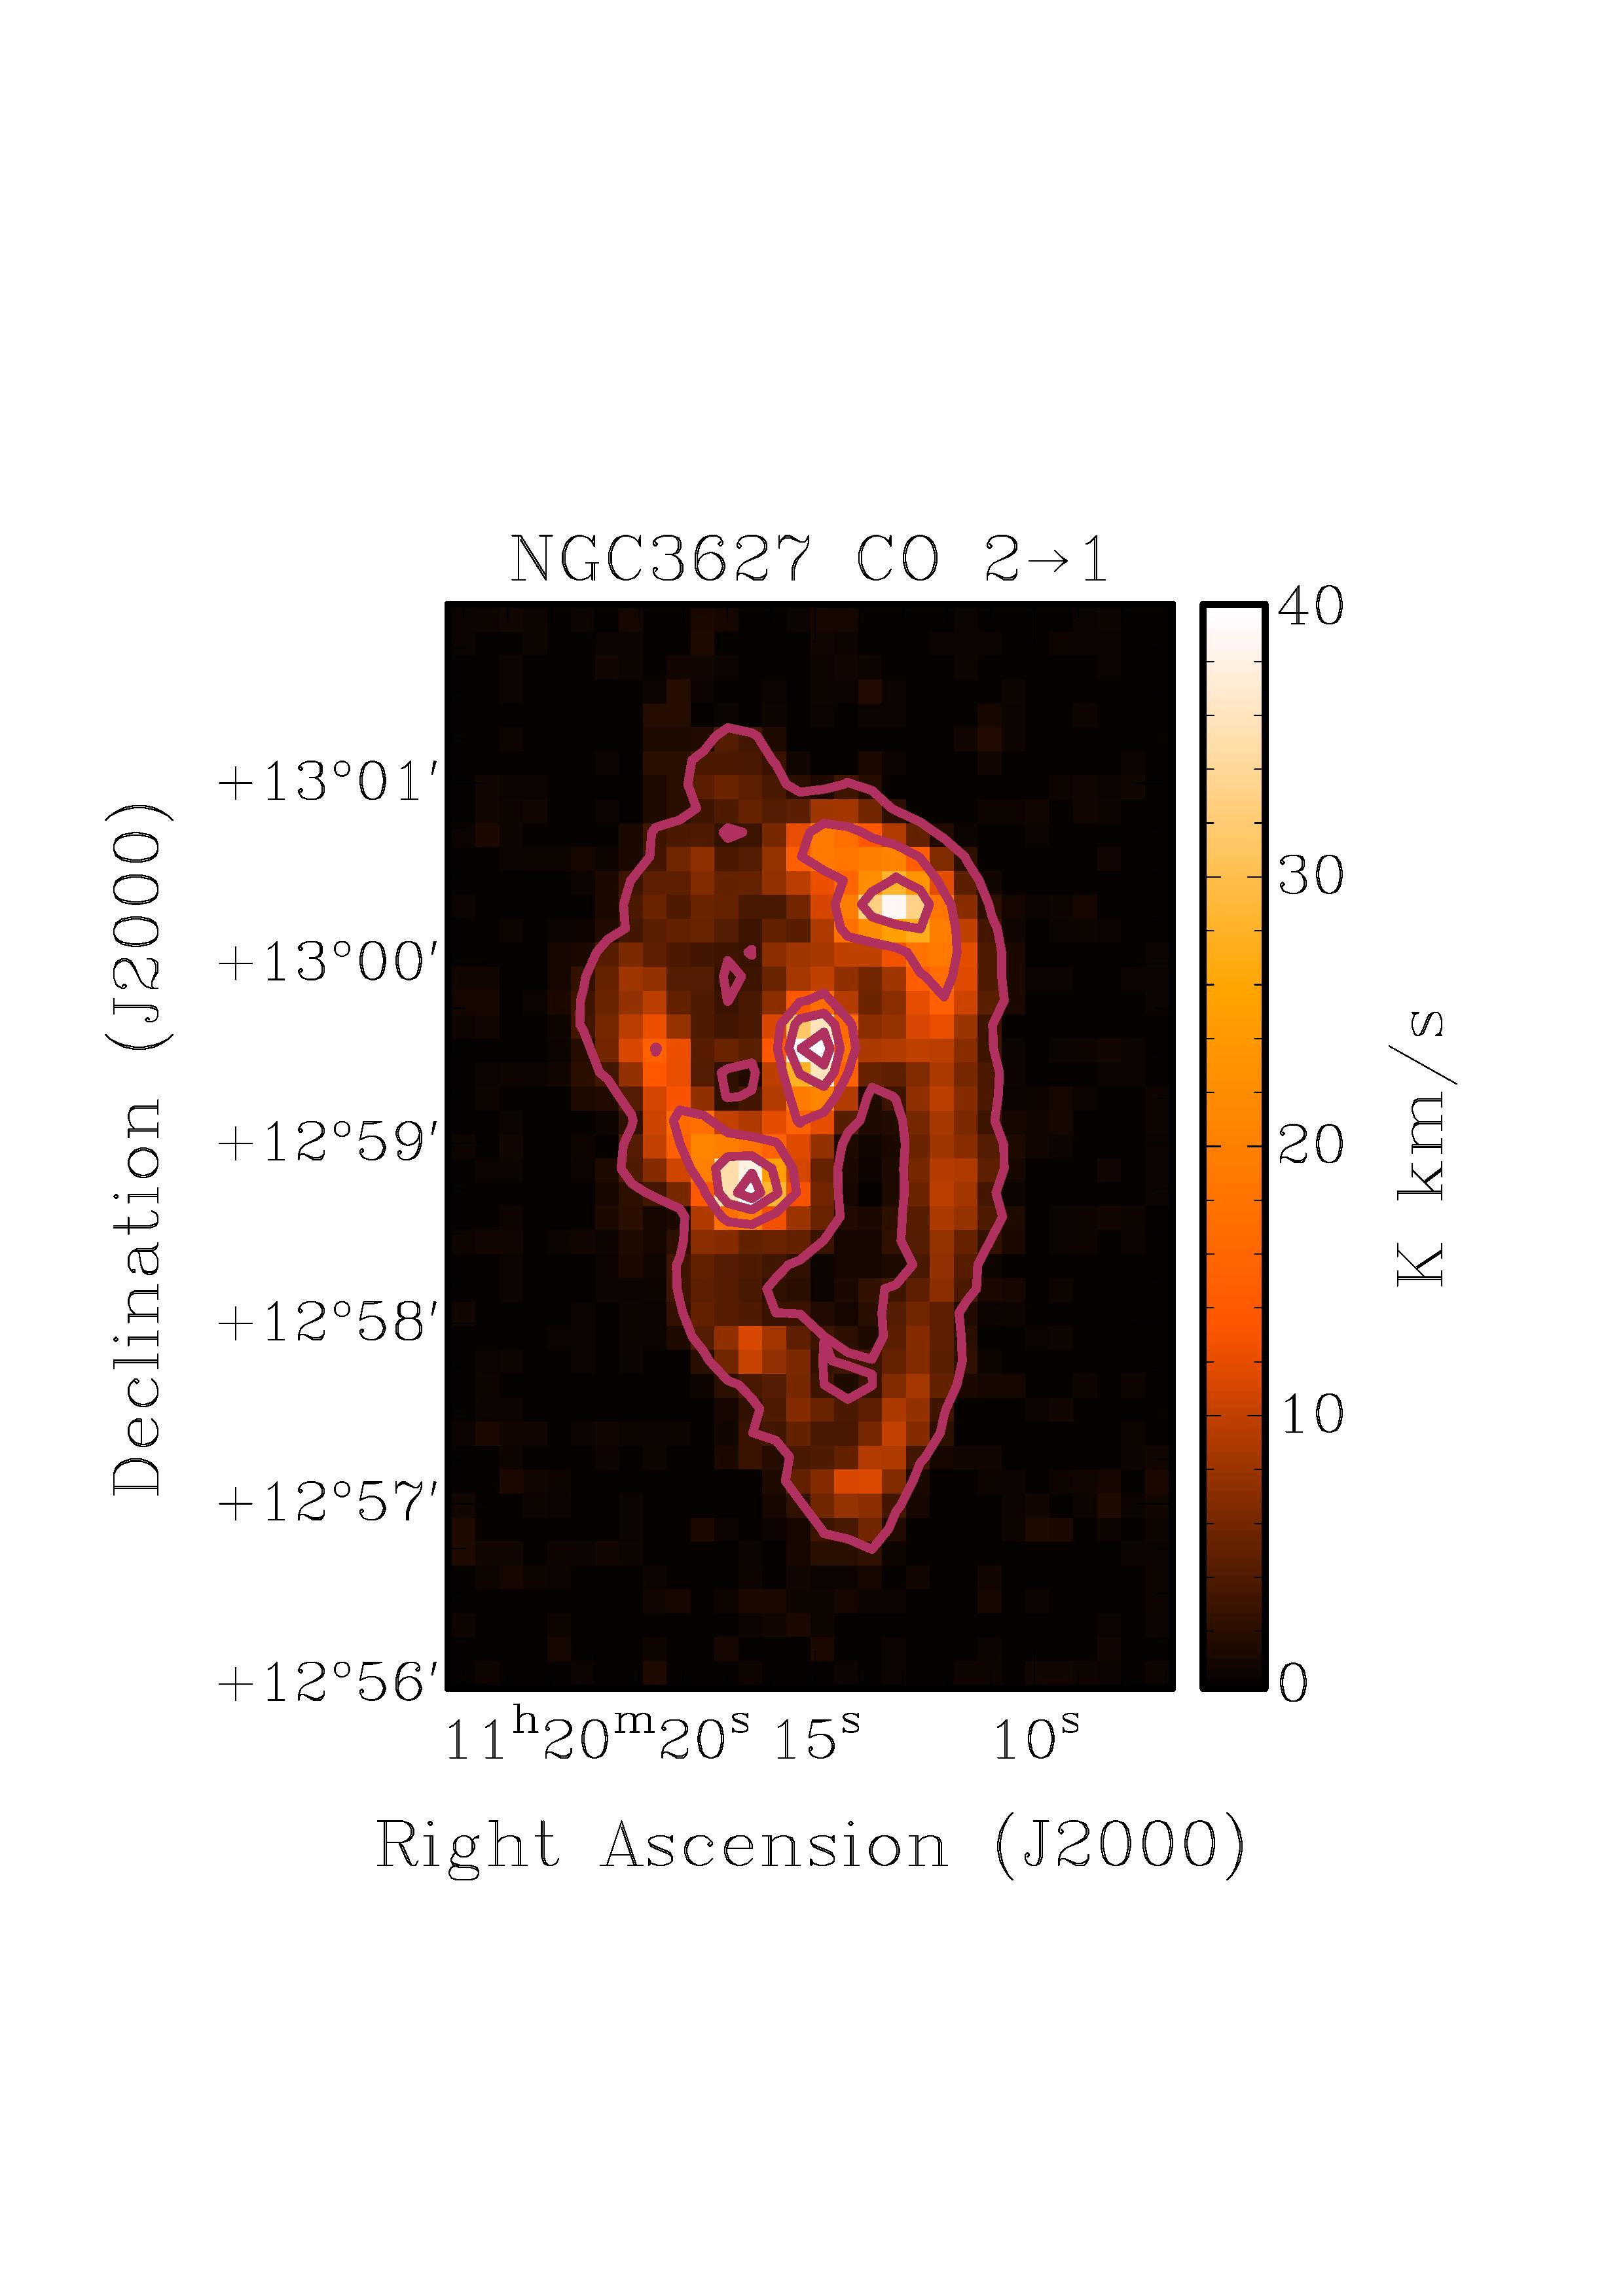
\includegraphics[scale=0.5]{obs_imgs/CO21.jpeg}
  \caption[NGC3627 $CO_{j=2-1}$ Observations]{Residual of the MAKEMAP filtering of $CO_{j=2-1}$ observations.}
\end{figure}

\begin{deluxetable}{cccc}
  \tablecolumns{4}
  \tablewidth{0pt}
  \tablecaption{Properties of NGC3627 HERACLES Observations\label{tab_obs_heracles}}
  \tablehead{\colhead{Observation} & \colhead{Beam Properties } & \colhead{RMS} & \colhead{Percentage of Emission Removed} \\
  & $\theta_{beam}$ & \it{[K km/s]}}
  \startdata
    $CO_{j=2-1}$ & 13.0$\arcsec$ & 0.305 & 7.8\% \\
  \enddata
\end{deluxetable}

\subsection{The HI Nearby Galaxy Survey (THINGS)}

To determine the gas to dust ratio we had to determine the total amount of gas present which required both atomic and molecular hydrogen.  We approximated the amount of molecular hydrogen present by using $CO_{j=1-0}$, and measured the amount of atomic hydrogen (HI) present.  The source of our atomic hydrogen came from The HI Nearby Galaxy Survey (THINGS) designed to observe HI emission in nearby galaxies with the extereme spatial resolution of the Very Large Array (VLA).  Targets in THINGS included many of the SINGS targets with the exception of known HI poor sources (E/S0 type galaxies), dynamicaly complex systems (edge-on spirals), and large extended galaxies found in the local group (\citet{walter2008}).

The preparation of the HI data was similar to the $CO$ filtering in the sense we did not convert the image into pW and let it remain in its native units.  The major difference in the HI extended emission filtering was we did not use a flux map for the final processing; instead we used a surface density map as our fakesource.  This was due to issues that arose when using the mass formula given in \citet{walter2008} on a filtered image.  Due to the high resolution of the VLA we measured significant losses in flux due to small scale structure after filtering.  The amount of lost structure for NGC3627 as a whole can be seen intable \ref{tab_obs_things} as well as the resolution, and rms of the filtered image.  The final data product is shown in figure \ref{fig_HI}.

\begin{figure}
  \centering
  \label{fig_HI}
  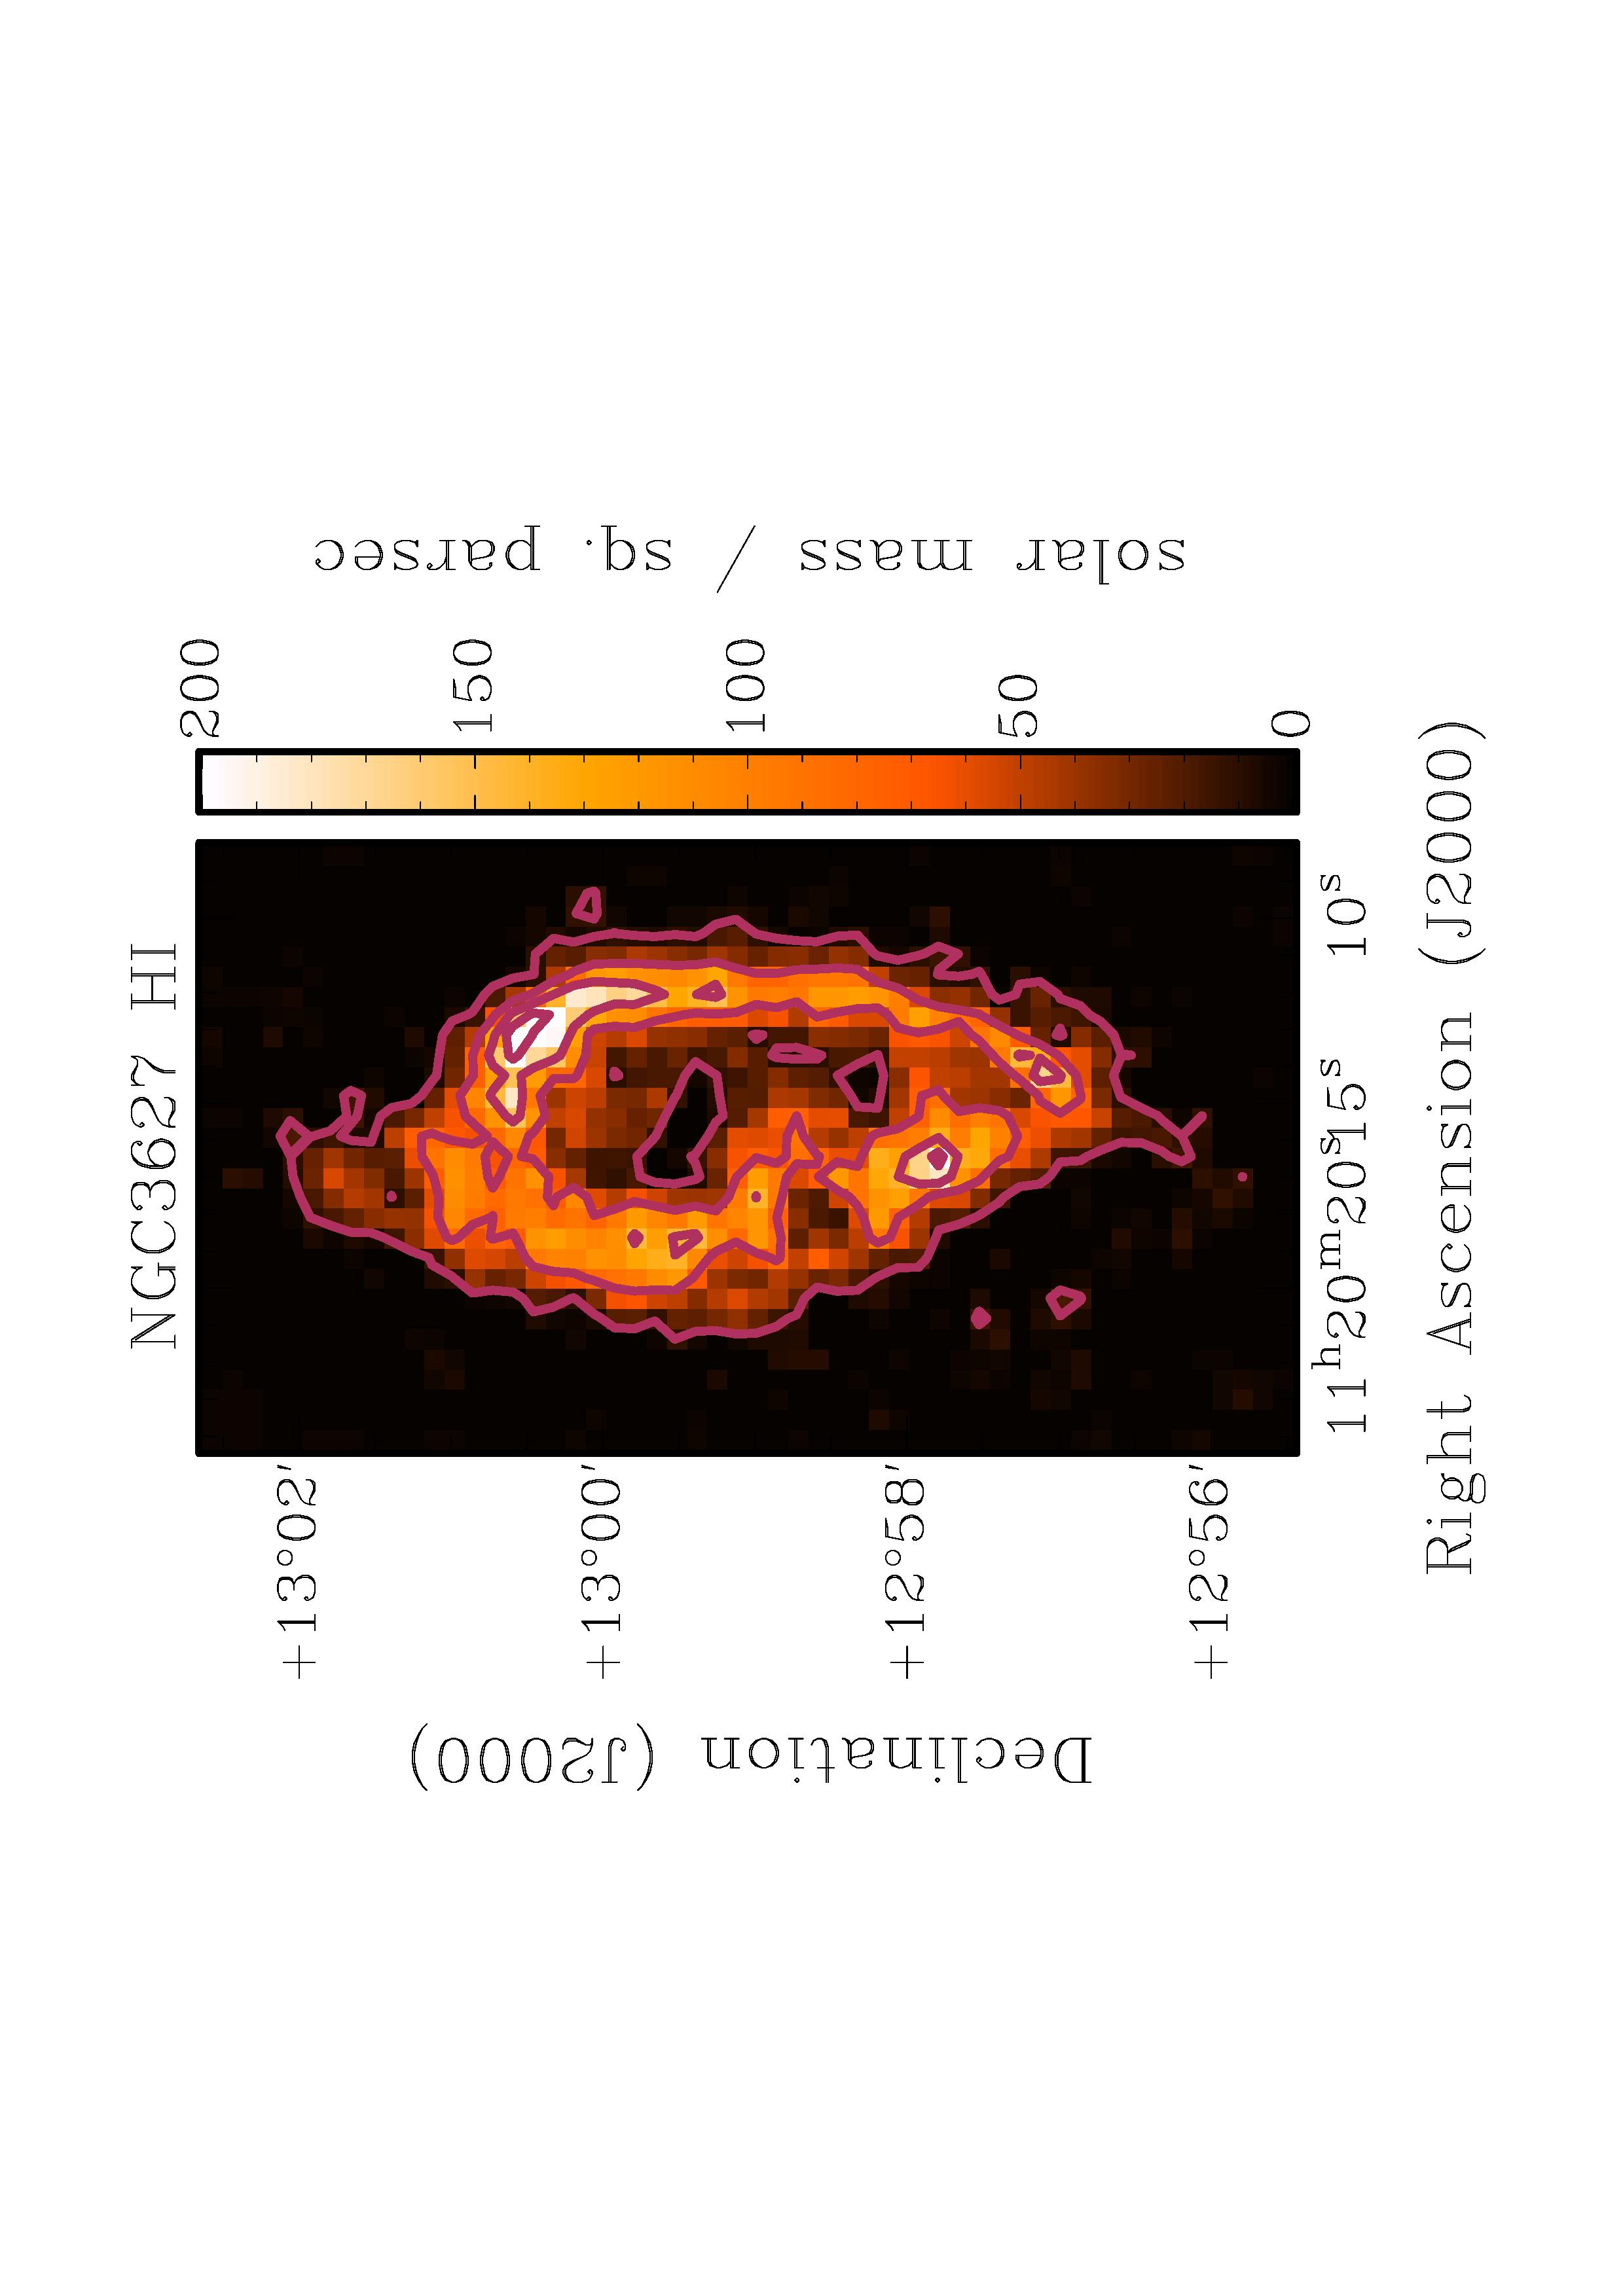
\includegraphics[scale=0.5,angle=270]{obs_imgs/HI.jpeg}
  \caption[NGC3627 HI Observations]{Residual of the MAKEMAP filtering of HI observations.}
\end{figure}

\begin{deluxetable}{cccccc}
  \tablecolumns{6}
  \tablewidth{0pt}
  \tablecaption{Properties of NGC3627 THINGS Observations\label{tab_obs_things}}
  \tablehead{\colhead{Observation} & \multicolumn{3}{c}{Beam Properties} & \colhead{RMS} & \colhead{Percentage of Emission Removed} \\
   & $\theta_{maj}$ & $\theta_{min}$ & $\theta_{PA}$ & \it{[$M_{\odot} / pc^2$]}}
  \startdata
    HI & 10.6$\arcsec$ & 8.85$\arcsec$ & -48.0$^\circ$ & 0.760 & 39.6\% \\  
  \enddata
\end{deluxetable}
